%!TEX root = Thesis.tex

\chapter{Rapid Layout Prototyping for Analog Design Migration}\label{chap:RLPADM}
  
  \section{Introduction}\label{sec:RLPADMIntro}

    In this chapter, we introduce the overall flow of the proposed layout migration methodology. Generally, analog design follows hierarchical design concept that produces structural design. 
    Hence, to extend the idea, we also consider the multilevel analog design in our prototyping framework. Figure~\ref{fig:Flow} shows the overall flow diagram. The flow is mainly separated into 3 stages: 1) the layout extraction and preservation stage, 2) the layout prototyping stage and 3) the wire segment refinement. 
    
    
    \begin{figure}[ht]
      \centering
      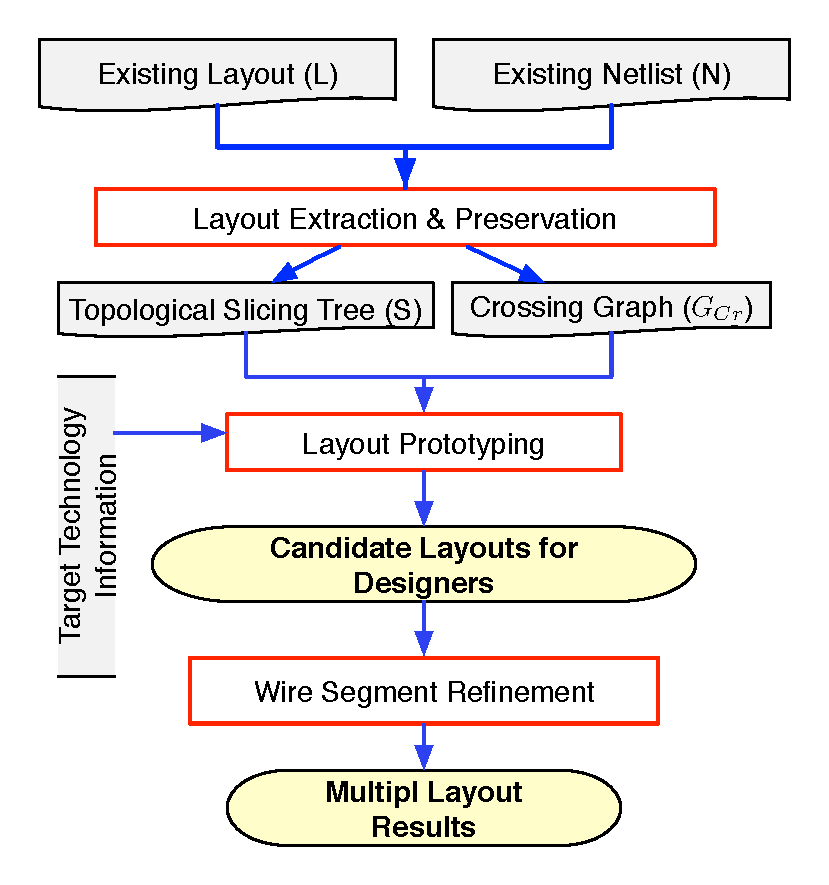
\includegraphics[width=0.5\textwidth]{Fig/Chapter4/Flow.eps}
      \caption{Overall flow of the proposed layout migration scheme.} 
      \label{fig:Flow}
    \end{figure}

    \begin{table}
      \begin{center}
      \caption{Comparison on Analog Layout Migration Approaches}\label{table:MigrateComp}
      \scriptsize
      \begin{tabular}{|c|c|c|c|c|}
        \hline
        & \cite{msc-bhattacharya-tcad06} & \cite{ALP_YPWeng_iccad2011} & \cite{Chin_DMR_ICCAD2013} & Our Approach \\
        \hline
        Layout Constraints & Preserved & Preserved & Preserved & Preserved \\
        \hline
        Placement topology  & Keep origin & Multi-prototypes & Already given & Multi-prototypes \\
        \hline  
        Routing behavior  & Partially preserved &  Manually completed &  Preserved routing & Preserved routing \\
        \hline
        \#Migrated Layout &  1 &  Multi-Solutions & Multi-Solutions & Wires refined Multi-Solutions \\
        \hline
        Sign-off Time &   slow &  slow &  fast &  fast \\
        \hline
      \end{tabular}
      \end{center}
    \end{table}

    In comparison with current migration mechanisms, Table~\ref{table:MigrateComp} shows the different criterion to examine the disparity. There are 3 current migration styles, \cite{msc-bhattacharya-tcad06}, \cite{ALP_YPWeng_iccad2011} and \cite{Chin_DMR_ICCAD2013}, mentioned in Table~\ref{table:MigrateComp}. For analog layout constraints, each approach is able to preserve specific constraints such as symmetry constraints and matching constraints. For placement topology, \cite{msc-bhattacharya-tcad06} aims to keep the exactly same topology as the existing layout, \cite{ALP_YPWeng_iccad2011} successfully produces multiple placement candidates and the placement in \cite{Chin_DMR_ICCAD2013} is already given. For routing behavior, \cite{msc-bhattacharya-tcad06} only preserves the wires that belong to the symmetric devices or clusters which are symmetric on the original layout, \cite{ALP_YPWeng_iccad2011} manually completes the routing section and \cite{Chin_DMR_ICCAD2013} quickly produces routing prototype with routing preservation. 

    Therefore, \cite{msc-bhattacharya-tcad06} generates single layout each time and \cite{ALP_YPWeng_iccad2011} can generate multiple layout solutions. \cite{Chin_DMR_ICCAD2013} produces multiple solutions from multiple placement results. To consider the Time-to-sign-off for overall flow, \cite{msc-bhattacharya-tcad06} and \cite{ALP_YPWeng_iccad2011} are slower due to the routing generation and \cite{Chin_DMR_ICCAD2013} facilitates the routing generation. In comparison, our approach consolidates the advantages from \cite{ALP_YPWeng_iccad2011} for more opportunity and \cite{Chin_DMR_ICCAD2013} for fast prototyping. Additionally, our approach refines the wires for better performance. In other words, we firstly generate multiple placement candidates and utilize them with preserved routing behaviors to fast generate multiple layout results. 

  \section{layout Preservation}\label{sec:LayoutPreserv}

    In this section, we emphasis on how to decompose the analog layout in placement and routing. We first divide the layout with blocks and wire segments, and later extract them respectively. The overall extraction flow is illustrated as Figure~\ref{fig:ExtractFlow}. 

    \begin{figure}[t]
        \begin{center}
          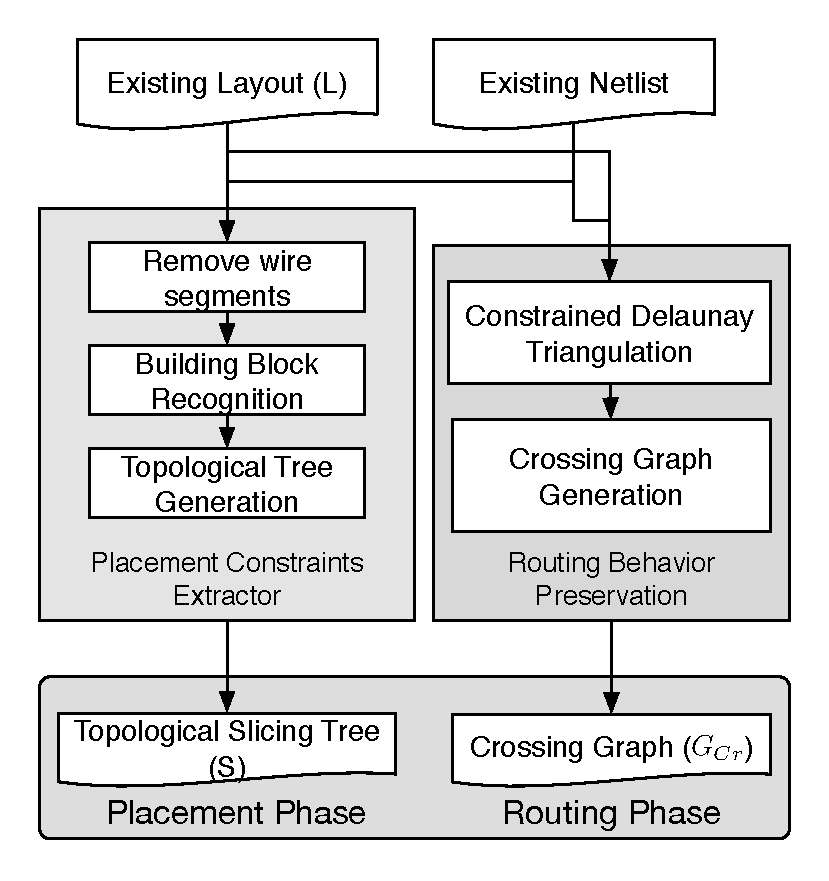
\includegraphics[width=0.7\textwidth]{Fig/Chapter4/ExtractFlow.eps}
          \caption{The extraction separates layout into placement phase as topological slicing tree and as routing phase crossing graph.}
          \label{fig:ExtractFlow}
        \end{center}
    \end{figure}
    \subsection{Placement Constraints Extraction}\label{sec:PlExtract}



      The major flow of placement constraints extraction \cite{ALP_YPWeng_iccad2011} is reviewed as follows:
      \subsubsection{Building Block Recognition}
        In order to reduce mismatch while generating layout, the principles of symmetrical and matching constraints should be considered as building blocks. 
        Besides, Building blocks under the same matching constraints are identified by the existing netlist. Via pattern matching technique \cite{srm-massier-tcad08} the preferable matching building blocks are generated.

      \subsubsection{Topological Slicing Tree Generation}
        Later, these fundamental build blocks construct the topological slicing tree. In general, the placement can be decomposed by horizontal and vertical cuts. However, since some of the devices are recognized as build blocks, the traditional slicing tree tends to occur mismatches. Instead, cells under the same building block are placed together as a super-module in representation. After vertical and horizontal  partitioning, a topological slicing tree (S) with n symmetry groups, m matching groups which outside any symmetry group, and l non-symmetry cells in layout are generated at the same hierarchy. Other than \cite{ALP_YPWeng_iccad2011} which flattens the layout into the unit hierarchy for slicing tree generation, we preserved the hierarchy of the layout with respect to the hierarchical structure from the existing netlist. Such hierarchy is essential for multi-level layout reconstruction. 
    \subsection{Routing Preservation via Crossing Graph Construction}\label{sec:CGC}

      This Section introduces a representation to preserve the routing correlation with placement. The routing preservation for analog layout is inspired from \cite{Chin_DMR_ICCAD2013}. We integrate the preservation strategy with placement accordingly. The routing channel can be decomposed into multiple triangles via CDT. Thus, the wire goes across one or more triangles on their edges. The representation which aims to record the "crossing" behavior among wires and triangular edges is denoted by a crossing graph. The crossing graph construction is demonstrated in the following paragraph. 

      \begin{figure}[t]
        \begin{center}
        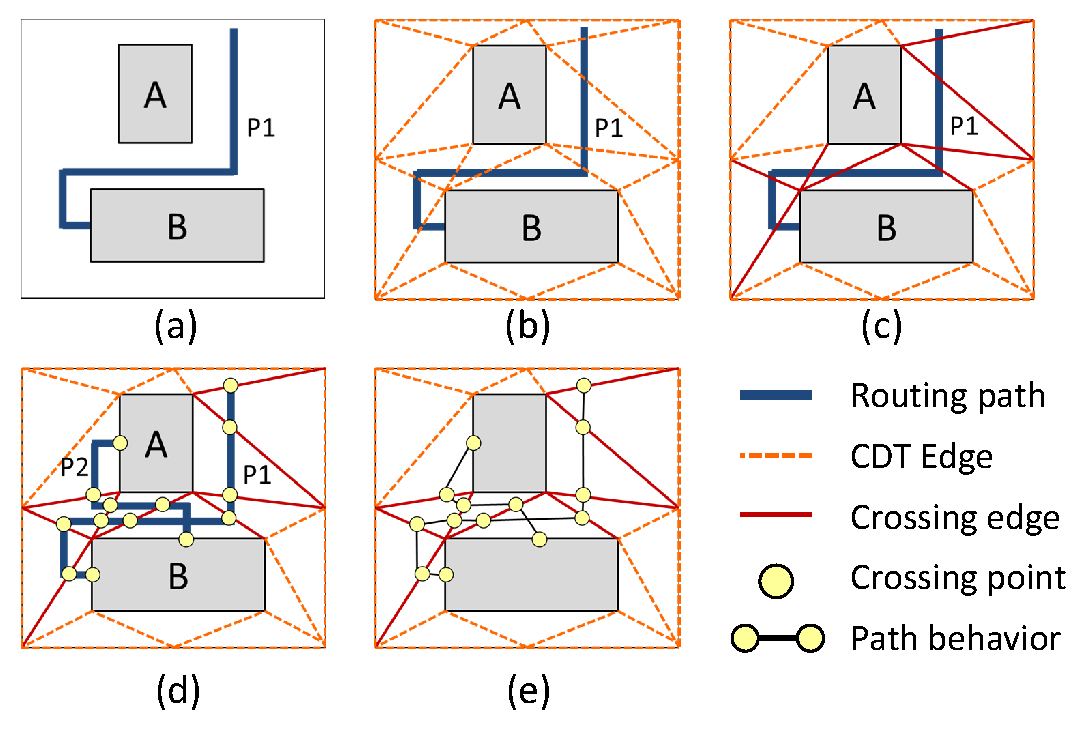
\includegraphics[width=0.7\textwidth]{Fig/Chapter4/CDT.eps}
        \caption{Illustration of routing preservation by CDT. 
          (a) The given design.
          (b) Resultant CDT graph.
          (c) CDT edges crossing with routing path are colored by red.
          (d) Crossing points of the two paths in routing plane.
          (e) Routing behavior is stored by CDT graph and the crossing points.}
        \label{fig:CGC}
        \end{center}
      \end{figure}

      Figure~\ref{fig:CGC} illustrates a routing preservation procedure. Given a layout plane $L$ with a set of placement blocks $B \in L$, where $B = \{b_i|1 \leq i \leq |B|\}$. As the layout without routing path shown in Figure~\ref{fig:CGC}.(a), the set of corner points of blocks in $B$ are denoted by $V_C$ where $V_C = \{(x_i,y_i)|1 \leq i \leq 4|B|\}$. We define the vertex set of the layout extraction CDT to be $V_{CDT} = V_C \cup V_{RP}$, and the points locate on the periphery of routing plane (i.e. corners of the routing plane and the middle-points of each routing plane boundary) are denoted by $V_{RP}$. Regions that forbid CDT edge are called {\it holes} in CDT formulations. In our case, they are the areas inside blocks and we use set $H$ to represent these holes. The CDT graph $G_{CDT}$ generated from vertex set $V_{CDT}$ and hole set $H$ can be represented as $G_{CDT} = \{V_{CDT},E_{CDT},T,H\}$, where edge set $E_{CDT} = \{(v_i,v_j)|v_i,v_j\in V_{CDT}\}$ splits the plane into a set of non-overlapping triangles $T$ and rectangular holes $H$.

      Through the CDT, the geometric correlation between blocks is recorded by the CDT edges as well as routing channels. Figure~\ref{fig:CGC} (a) is a layout diagram with two blocks and one routing path, and Figure~\ref{fig:CGC}(b) shows the CDT graph generated by the layout, where $|V_{CDT}|=16$, $|H|=2$ (holes A and B), $|E_{CDT}|=34$ and $T=18$. 

      The solid red lines denote CDT edges that are crossing with the routing path in Figure~\ref{fig:CGC}(c). Through the triangulation, the routing plane is divided into a set of non-overlapping triangles with each edge representing a geometric relation between blocks. The path behavior can thus be recorded as an ordered set of CDT edges being crossed by that path.

      After $G_{CDT}$ is established, one routing path is recovered back to demonstrate the routing preservation. As displayed in Figure~\ref{fig:CGC}(c), one $e_{CDT}$ intersects with the routing path is denoted by a crossing edge $e_{Cr}$ and the intersected point is denoted by a crossing point $v_{Cr}$. The detailed definition is as follows.

      \begin{defi}\label{defi:CrossingPoint}
        Given a routing path $p$, and CDT edge set $E_{CDT}= \{e_{CDTi}| 1 \leq i\leq|E_{CDT}|\}$, if there exists a point $v(x,y)$ which is both on $p$ and $e_{CDTi}$, $e_{CDTi}$ is a crossing edge $e_{Cr}$ and $v(x,y)$ is a crossing point $v_{Cr}$.
      \end{defi}

      \begin{figure}
        \begin{center}
        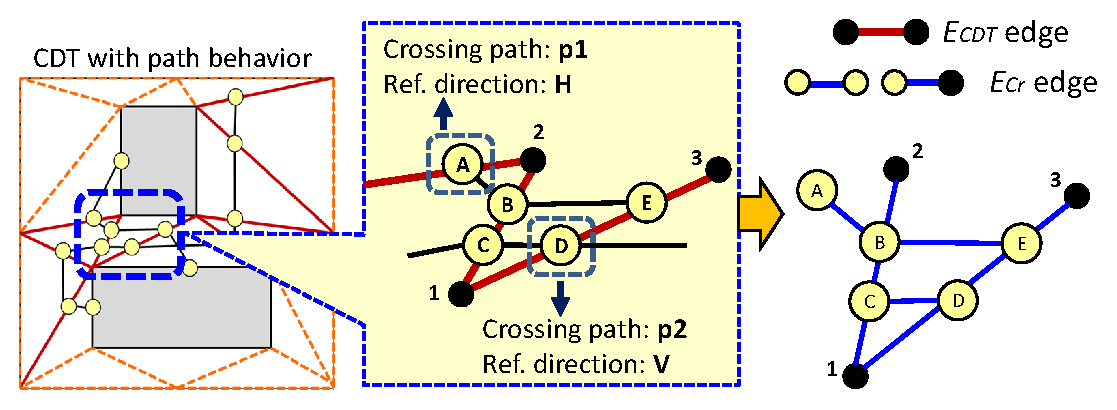
\includegraphics[width=0.7\textwidth]{Fig/Chapter4/CrG.eps}
        \caption{Illustration of crossing graph generated from Figure~\ref{fig:CGC}(d).
          $V_{Cr}$ points store the path direction as reference direction in routing reconstruction stage, 
          and $E_{Cr}$ edges are constructed to connect (1) adjacent points on the same CDT edge and (2) adjacent points on the same path.}
        \label{fig:CrG}
        \end{center}
      \end{figure}


      For multiple nets design, a single edge might be crossed with two or more routing paths. As illustrated in Figure~\ref{fig:CGC}(d), the two routing paths, $p1$ and $p2$, both pass through space between block A and B with p2 closer to block A. In order to preserve the behavior of multiple nets routing, we define the {\it crossing graph} $G$ of layout $L$ as follows: 

      \begin{defi}\label{defi:CrossGraph}
        Let $G_{CDT}(V_{CDT},E_{CDT},H,T)$ denotes the CDT graph of $L$. $V_{Cr}$ denotes the set of crossing point and $E_{Cr}$ denotes the set of crossing edges. Then graph $G_{Cr} = \{V_{CDT} \cup V_{Cr},E_{CDT} \cup E_{Cr},H,T\}$ is a crossing graph of layout $L$. 
      \end{defi}

      In the end, the crossing graph stores not only the individual routing topology, but also the relative order of paths within each routing channel.

    \subsection{Hierarchical Layout Extraction and Preservation}\label{sec:HLE}

      \begin{figure}[t]
        \begin{center}
        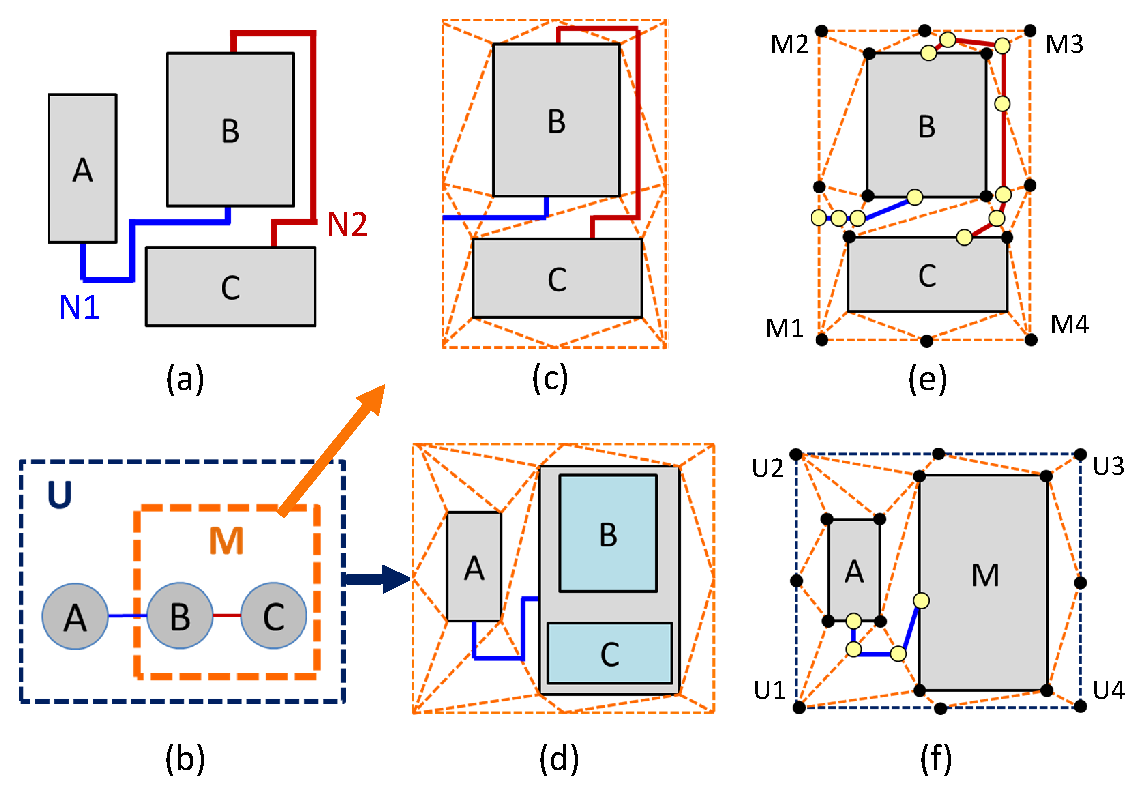
\includegraphics[width=\textwidth]{Fig/Chapter4/HIER.eps}
        \caption{
           (a) A layout with 3 placement blocks and two routing paths. 
           (b) Hierarchical Structure of (a).
           (c) CDT graph of cluster M (bottom level cluster).
           (d) CDT graph of cluster U (upper level cluster).
           (e) Corresponding crossing graph of (c).
           (f) Corresponding crossing graph of (d), cluster M is regarded as a placement block here.
          }
        \label{fig:HIER}
        \end{center}
      \end{figure}

      In order to reduce mismatches, the symmetry and proximity constraints need to be considered for both placement and routing. 
      For the given source layout, modules/devices are grouped as clusters according to the symmetry and proximity constraints, 
      where the constraints can be either given by designers or extracted from the source layout as in Section~\ref{sec:PlExtract}.

      For each cluster, the routing behavior and correlation with placement blocks are analyzed based on the CDT of that cluster to build a corresponding crossing graph. 
      Crossing graphs of clusters are constructed bottom-up along the hierarchical structure. 
      Bottom-level clusters are regarded as placement blocks in upper-level clusters. 
      Consequently, a series of crossing graphs is generated which contain the routing behavior hierarchically.

      Figure~\ref{fig:HIER} illustrates this multilevel crossing graph generation.
      Figure~\ref{fig:HIER}(a) shows a simple layout with three blocks and two nets.
      Assume block B and C are grouped into cluster M, and M and A are grouped into U as shown in Figure~\ref{fig:HIER}(b).
      According to the hierarchy, two crossing graphs are constructed with respect to cluster M and U, and
      each routing path is divided into 1) intra-cluster connections and 2) inter-cluster connections. 
      As illustrated in Figure~\ref{fig:HIER}(c)(d), path N1 is segmented into inside parts and outside parts of M. 
      Therefore, the crossing points of N1 appear in both two crossing graphs. 
      On the other hand, since N2 contains only intra cluster connection in M, the corresponding crossing points are all inside a single graph.

  \section{Prototyping}\label{sec:Proto}

    \begin{figure}[t]
      \centering
      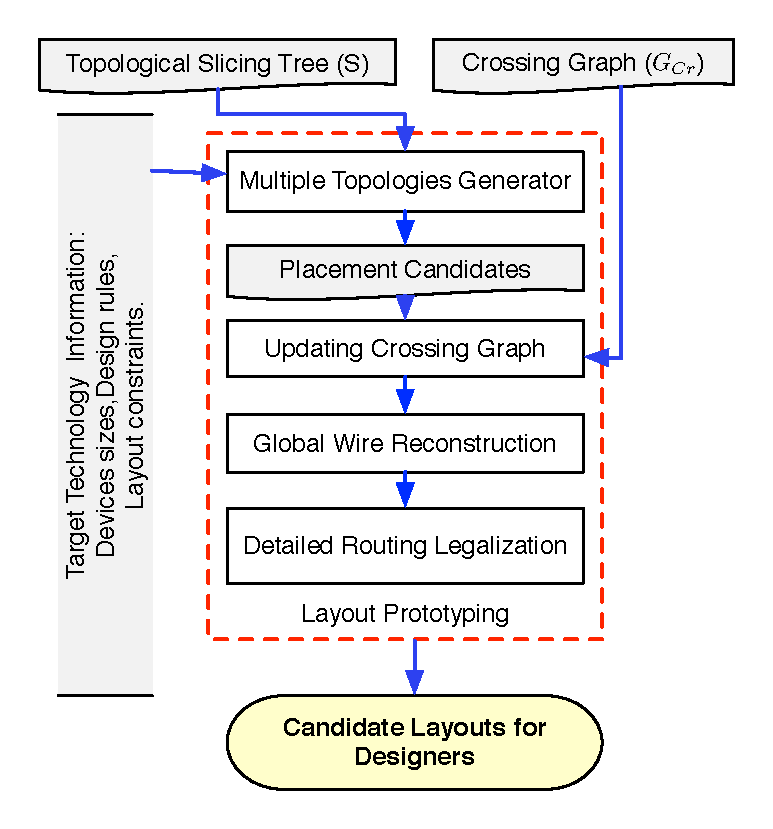
\includegraphics[height=0.7\textwidth]{Fig/Chapter4/Proto_Flow.eps}
      \caption{Flow of the proposed layout prototyping scheme.} 
      \label{fig:Proto_Flow}
    \end{figure}

    In this section, a prototyping flow is proposed as Figure~\ref{fig:Proto_Flow} illustrated. We first update the technology information for placement blocks and routing components. Later, the set of placement results are obtained by \textit{Multiple topologies generator} according to the extending DeFer in~\cite{ALP_YPWeng_iccad2011}. Multiple placement results which use the same hierarchical structure in Section~\ref{sec:HLE}. Mostly, the updated topologies of placement are changed. Once the placement topology is updated, the corresponding routing behavior should also be updated. The correlation between placement and routing is preserved as a crossing graph via CDT. Therefore, the crossing graph needs to be updated so that the routing can be reconnected correctly. Section~\ref{sec:updateG} adopts the updating methodology from \cite{Chin_DMR_ICCAD2013}, which further considers the routing direction changing in the migrated layout. The routing is generated on each of the placement candidate automatically by a bottom-up manner in Section~\ref{sec:GWRecon} and Section~\ref{sec:DRLegal}. 

    \subsection{Crossing Graph Updating}\label{sec:updateG}


      In order to obtain routing in the targeting placement with similar behavior to source layout, we update the crossing graph $G$ of each cluster into new placements which are generated from {\it Multiple Topologies Generator}. The objective motivation is to reflect the change of placement. Once the placement is changed, the coordinate of corners of blocks are changed as well. Since the locations of vertices are different from the original $G_{CDT}$, the updated graph $G'_{CDT}(V'_{CDT},E'_{CDT},T',H')$ is generated according to the new position/size of placement blocks. Figure~\ref{fig:updateG}(a) shows the original CDT graph $G_{CDT}$ of two placement blocks and the changed graph $G'_{CDT}$. This graph has the same number of vertices, edges, triangles, and holes with $G_{CDT}$, but with different vertex coordinates. $G'_{CDT}$ is no longer a CDT graph since its edges and triangles are distorted from the original one. (It is like the original graph being stretched.) Some edges might overlap with placement blocks, which are represented as solid red line in Figure~\ref{fig:updateG}(a).


      \begin{figure}[ht]
        \begin{center}
        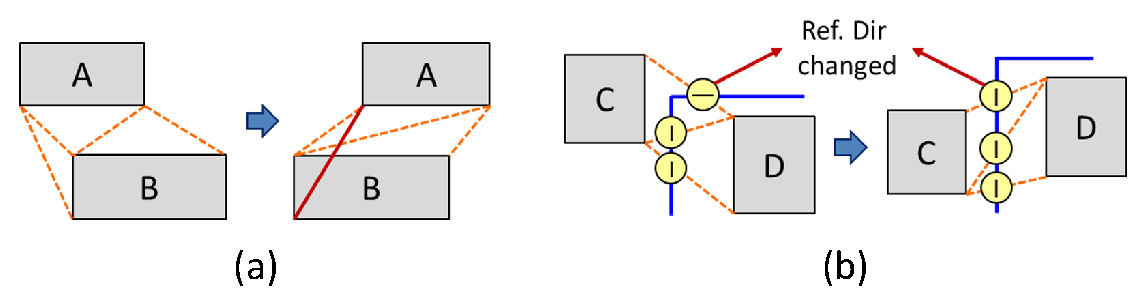
\includegraphics[width=0.7\textwidth]{Fig/Chapter4/updateG.eps}
        \caption{
          Updating crossing graph to reflect placement change.
          (a) Illustration of edge invalidation (solid red line) due to overlapping with blocks.
          (b) Illustration of changing reference direction of a crossing point.
          }
        \label{fig:updateG}
        \end{center}
      \end{figure}


      Notice that once an edge overlaps with blocks in graph $G'_{CDT}$, it actually reveals the correlation vanished between placement blocks, which means the edge no longer represents a routing channel. These overlapping edges are set to be {\it invalid} to indicate that the routing information stored on this edge is incorrect. According to Figure~\ref{fig:updateG}.(a), the crossing graph is updated by removing the invalid crossing edges and the invalid crossing point on them. This operation reflects the placement updating. On the contrary, if there does not exist any overlapping between edges and blocks in $G'_{CDT}$, the routing behavior can be well preserved even if the layout changes.


      The reference directions stored on crossing points give a superb hint when reconstructing routing paths on a different placement.
      In certain cases, the direction should be changed from H to V (or V to H) due to the slope of CDT edge varies. As illustrated in Figure~\ref{fig:updateG}.(b), there are three crossing points, two of them have direction V and the top one has direction H. After changing the placement, every $CDT$ edge remains valid (no overlapping with holes). However, the direction of the top most crossing point cannot be changed into horizontal due to the y direction vector of the corresponding CDT edge changed from negative to positive. If such situation occurs, the reference direction will be changed from H to V. We further discuss the conditions that are supposed to happen while updating crossing edge.

       
      \begin{figure}[t]
        \begin{center}
          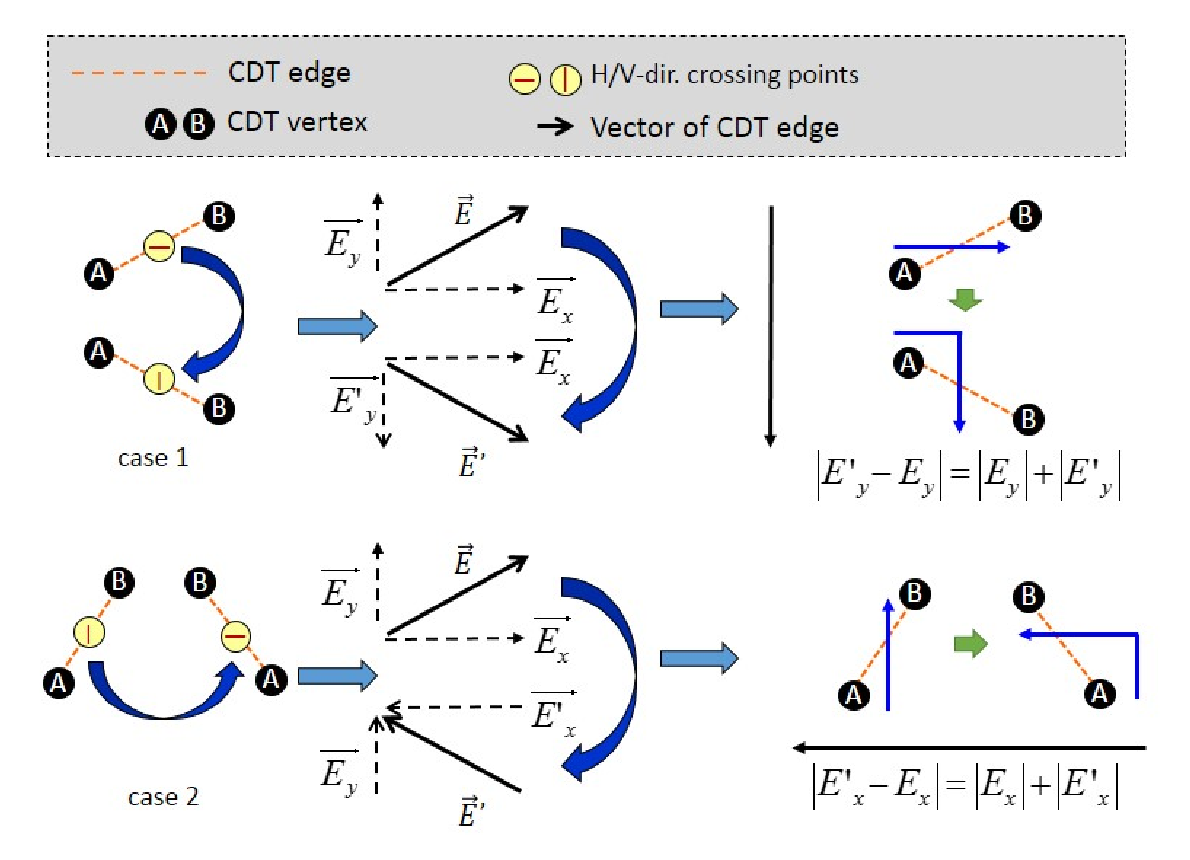
\includegraphics[width=0.7\textwidth]{Fig/Chapter4/refdir2.eps}
          \caption{Reference direction updating due to angle changing of CDT edge.
           In case 1, H-direction crossing points are updated to V. 
             In case 2, V-direction crossing points are updated to H.}
          \label{fig:refdir}
        \end{center}
      \end{figure}

      The situation is generalized into two cases as listed in Figure~\ref{fig:refdir}.
      For a CDT edge $E$, assume the two endpoints are vertex A and vertex B. Without loss of generality, we consider edge E as a vector $\overrightarrow{E}$, which can be decomposed into x-direction vector $\overrightarrow{E_x}$ and y-direction vector $\overrightarrow{E_y}$. According to Figure~\ref{fig:refdir}, case 1 and 2 are demonstrated for reference direction changing as follow, 


      \begin{enumerate}
        \item For a case that the difference of y-direction vector between $\overrightarrow{E}$ and $\overrightarrow{E'}$ equals the sum of both y-direction vectors' modulus, where $|\overrightarrow{E_y'} - \overrightarrow{E_y}|=|\overrightarrow{E_y'}|+|\overrightarrow{E_y}|$. It indicates that the vertical direction of the updated CDT edge is opposite to the origin. Therefore, if the reference direction of the crossing edge is horizontal primitively, it should be updated to vertical for path extension.
        \item For a case that the difference of x-direction vector between $\overrightarrow{E}$ and $\overrightarrow{E'}$ equals the sum of both x-direction vectors' modulus, where $|\overrightarrow{E_x'} - \overrightarrow{E_x}|=|\overrightarrow{E_x'}|+|\overrightarrow{E_x}|$. It indicates that the horizontal direction of the updated CDT edge is opposite to the origin. Therefore, if the reference direction of the crossing edge is vertical primitively, it should be updated to horizontal for path extension.
      \end{enumerate}

    \subsection{Global Wire Reconstruction By Orthogonal Segments}\label{sec:GWRecon}
      For each cluster $i$ of input design, we re-construct routing paths according to the corresponding crossing graph $G_{Cri}$.
      Recall that each crossing point $v \in V_{Cr}$ in $G_{Cri}$ is with a reference direction stored on it.
      For each $G_{Cri}$, the orthogonal wire segments are generated as follows:
      (a) adjacent crossing points with the same reference direction are aligned to produce a set of vertical/horizontal segments.
      (b) if step (a) does not produce illegal routing such as crossing with other modules/devices, it will be preserved, else
      (c) the program will split the segment into several sub-segments with each sub-segment can be routed using the reference direction legally, and then we connect these sub-segments using pattern route.
      (d) wire spacing constraint of each metal layer are examined and adjusted by shifting segments.


    \subsection{Detailed Routing Legalization}\label{sec:DRLegal}
      Once the routing reconnection of all bottom level clusters are complete, 
      these clusters are regarded as placement blocks in the upper level,
      and the wire segments connected to the block boundary are taken as pin locations in the upper level.
      The procedure is repeated until the top-level design of routing is obtained.

    Since all the above steps are implemented automatically, each net still needs to be patched in detail. For instance, the pin connections inside the devices are done manually since the location inside each devices are changed from the source layout to the target technology. 
    However, since we perform detailed routing legalization scheme in a comprehensive view, most of the tasks are covered and the detail refinement is easier to implement for analog layout designers.
  
  Note that the routing behaviors are generally preserved in the targeting layout due to the similarity among the original placement and the targeting placement. Thus, the preservation of routing is flexible. The fundamental idea of routing preservation in this paper is to preserve the corresponding wires with the placement topology. If the designers decide to select a different placement topology, the necessity of preservation for routing is less. Hence, that is what our triangulation-based preservation provides.


  \section{Wire Segment Refinement}\label{sec:WSR}

    \begin{figure}[t]
      \centering
      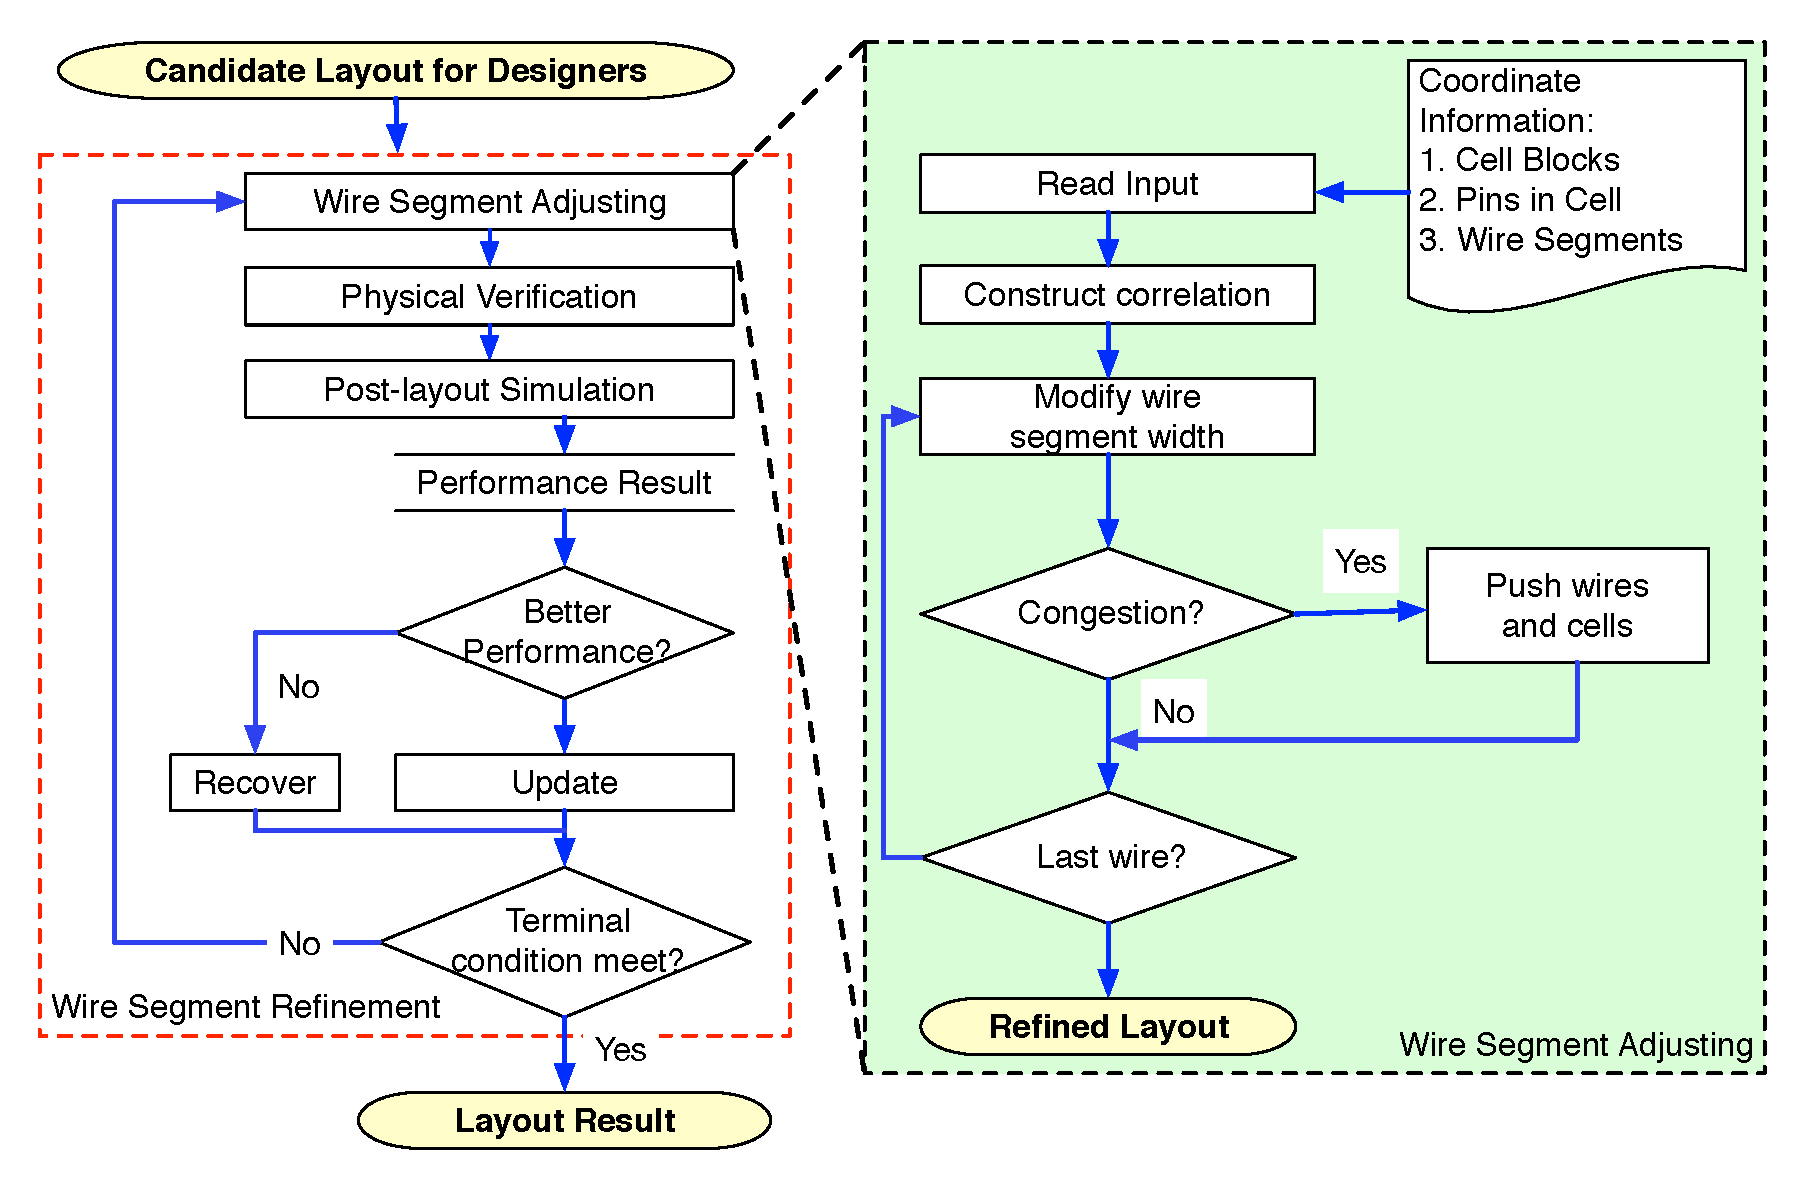
\includegraphics[width=\textwidth]{Fig/Chapter4/WireSegRefine.eps}
      \caption{Flow of the proposed Wire Segment Refinement.}
      \label{fig:WireSegRefine}
    \end{figure}
    
      


    After the prototypes of targeting layout is generated, these can be verified by design rules and post-layout simulation for manufacturing. In addition, our flow refines the routing on wire segments. Considering the resistant effect from wire segment, different width of each segment results in different unit resistance on routing. Practically speaking, the wires cannot be extended as wide as possible due to the limited area and design for manufacturing factors, which are relevant to advanced technologies. In this stage, our methodology traverses a solution under limited area with refined wire segments automatically. We practice a simulated annealing flow in Figure~\ref{fig:WireSegRefine} to perturb the optimal solution for wire segments.

    
    

    According to {\it Wire Segment Adjusting} in Figure~\ref{fig:WireSegRefine}, a set of segments is selected to change the width in each iteration and then the performance result is evaluated . Gathering the information of coordinate position and size of cell, every pin's location for each cell and the fixed block, is the prerequisite for the program. After having the information stored, finding the correlation of wires and cells becomes a chief task. The correlation should be established in horizontal and vertical respectively in each layer. For every layer, the routing wires are avoided overlapping on the cell area because of the possibility of crosstalk and unexpected error. The spaces left for horizontal (vertical) wires on upper and lower (left and right) directions are checked to obtain the preferred direction. Moreover, the trivial expansion of routing area can be avoided. 

    Later, we update the width of the targeting wire segment and then check the occurrence of any congestion. For every single step in simulated annealing, two wire segments are chosen randomly for updating. We increase one segment's width and decrease another. Since the area of the overall layout is fixed, the capacity for each segment is also limited. Changing the width of each wire segment makes congestion to be occurred easily. Once a congestion happens among blocks or wire segments, these wires or blocks are recursively pushed away from the congested area.

    Figure~\ref{fig:Congestion} demonstrates one example for conducting the congestion elimination recursively. As soon as all the congestions are eliminated, the adjusting flow keeps changing the rest wires' width until there is no wire for adjusting. The refined layout with updated wire proceeds to physical verification. As the layout passing physical verification and the performance of such circuit is obtained by post-layout simulation. This layout is chosen based on possibility P which is related to the difference of the performance, the cooling-down temperature and the annealing factor to reduce the temperature. In the end, the layout with updated wires is generated.
    \begin{figure}[t]
      \centering
      \centerline{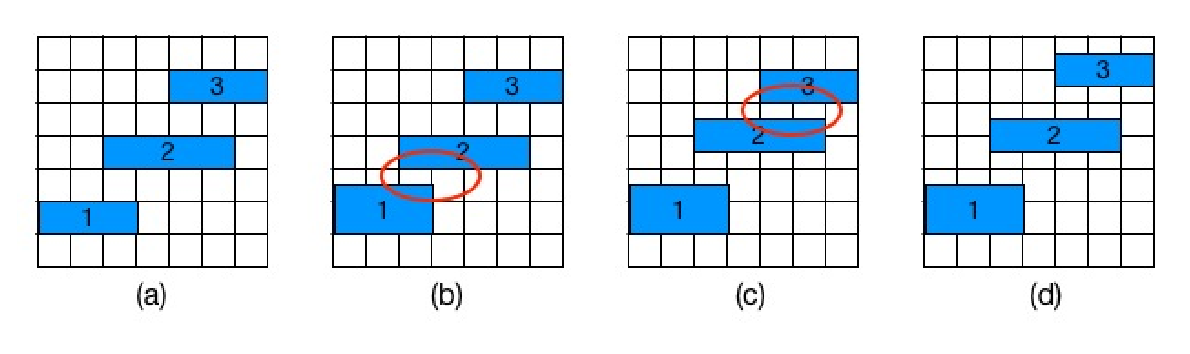
\includegraphics[width=\textwidth]{Fig/Chapter4/Congestion.eps}}
      \caption{Example of recursively segment pushing. (a) original layout. (b) Widened segment 1 and congestion occurs. (c) Pushing segment 2 above to avoid congestion between 1 and 2 but another congestion occurs among 2 and 3. (d) Pushing segment 3 above and then congestion eliminated.} 
      \label{fig:Congestion}
    \end{figure}


  \section{Experimental Results}\label{sec:RLPADMExp}

    Our layout migration framework is implemented in c++ language on Intel 5420 Quad Core 2.5GHz machine under Linux CentOS 5.8 platform. We apply OpenAccess v22.04p54 for extracting industrial design and using Synopsys PyCell Studio for layout generation. Three experimental circuits are practiced as our reference layouts: (1) A folded-cascode operational amplifier (OpAmp) design, (2) a variable-gained amplifier (VGA) under umc90nm, and (3) a low drop-out regulator (LDO). 

    \begin{table}[ht]
      \scriptsize
      \begin{center}
        \caption{Invalid crossing edges and crossing points of migrated crossing graph comparing to original crossing graph}\label{table:CrEdgeChanged}
        \begin{tabular}{|c|c|c|c|c|m{1.2cm}|}
          \hline
            Tech. & layout & \#Invalid CrEdge & \#Invalid CrPoint\\
          \hline
          \rowcolor{mygray}
          \multicolumn{4}{|c|}{Opamp: \#TriEdge=150, \#CrEdge=83, \#CrPoint=193} \\
          \hline
          \multirow{8}{*}{umc65nm} & Topo1 & 0 & 0 \\
          \cline{2-4}
          & Topo2 & 31 & 23 \\
          \cline{2-4} 
          & Topo3 & 20 & 10 \\
          \cline{2-4}
          & Topo4 & 0 & 0 \\ 
          \cline{2-4}
          & Topo5 & 24 & 37 \\
          \cline{2-4}
          & Topo6 &15 & 24\\
          \cline{2-4}
          & Topo7 & 46& 61 \\
          \cline{2-4}
          & Topo8 & 11 & 15 \\
          \hline
          tsmc90nm & Topo1 & 4 & 11 \\
          \hline
          \rowcolor{mygray}
          \multicolumn{4}{|c|}{VGA: \#TriEdge=353, \#CrEdge=249, \#CrPoint=810} \\
          \hline
          umc65nm & Topo1 &  95 & 298 \\
          \hline
        \end{tabular}
      \end{center}
    \end{table}

    In the following experiments, we intend to show the ability of layout reusability by our migration flow. Therefore, we compare several migrating techniques as below: 

    \begin{itemize}
      \item {\bf \cite{msc-bhattacharya-tcad06}}: Placement migrated into targeting technology and the corresponding routing is accomplished by manual routing.
      \item {\bf \cite{ALP_YPWeng_iccad2011}}: Placement migrated into targeting technology with multiple topologies. The producing placements partially preserved the constraints including symmetry, matching and proximity with respect to the original layout.
      \item {\bf \cite{Chin_DMR_ICCAD2013}}: Routing migrated into targeting technology based on CDT preservation. If the topology of placement changes, the relationship among wires and modules can be partially preserved and reconnected.
      \item {\bf RtMaMi}: Routing manually migrated into targeting technology. 
      \item {\bf RtNoMi}: Routing is not migrated into targeting technology. A simple maze routing is applied to connect the wires. 
      \item {\bf Ours:}  Our approach is a mixed version of \cite{ALP_YPWeng_iccad2011}, \cite{Chin_DMR_ICCAD2013} and {\it Wire Segment Refinement} which is implemented for better performance.
    \end{itemize}

    We first practice the proposed migration framework to layout generation towards different technologies in Section~\ref{sec:ExpMigration}. Later, a comparison among multiple migrated placements with different routing migrating techniques is demonstrated in Section~\ref{sec:ExpMultiProto}. The specifications of the source layouts for OpAmp and VGA in Section~\ref{sec:ExpMigration} and Section~\ref{sec:ExpMultiProto} are the same as Table I in \cite{Chin_DMR_ICCAD2013}. In addition, Table~\ref{table:CrEdgeChanged} notes the number of invalid crossing edge and invalid crossing point for each layout after migration. In brief, the fewer invalid crossing edges and invalid crossing points, the more reusability of the updated crossing graph.


    \begin{figure}[ht]
        \centering
          \begin{subfigure}[t]{0.4\textwidth}
          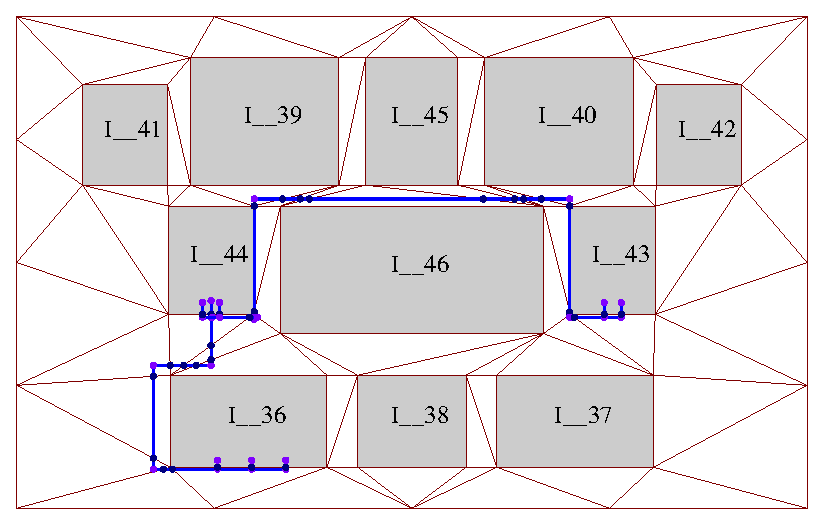
\includegraphics[width=\textwidth]{Fig/OrigOpamp.eps}
          \caption{OpAmp umc90nm}\label{fig:OrigOpamp}
          \end{subfigure}
          \begin{subfigure}[t]{0.4\textwidth}
          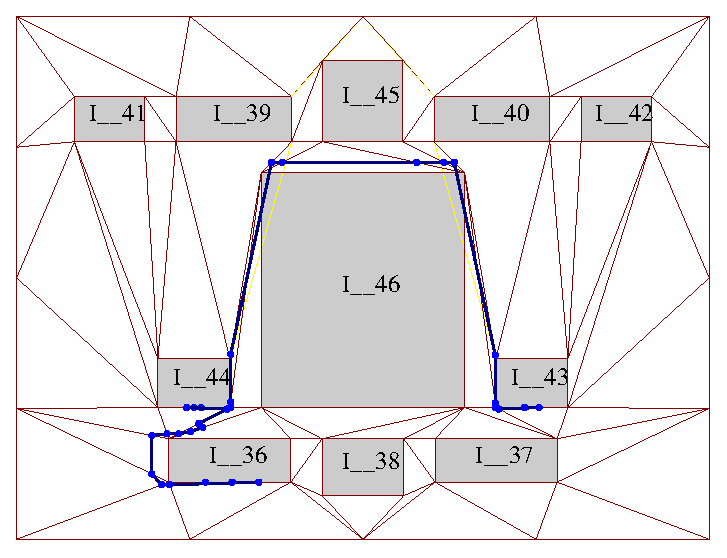
\includegraphics[width=\textwidth]{Fig/OpampProto.eps}
          \caption{OpAmp tsmc90nm}\label{fig:OpampProto}
          \end{subfigure}
          \begin{subfigure}[t]{0.4\textwidth}
          \includegraphics[width=\textwidth]{Fig/OrigVGA.eps}
          \caption{VGA umc90nm}\label{fig:OrigVGA}
          \end{subfigure}
          \begin{subfigure}[t]{0.4\textwidth}
          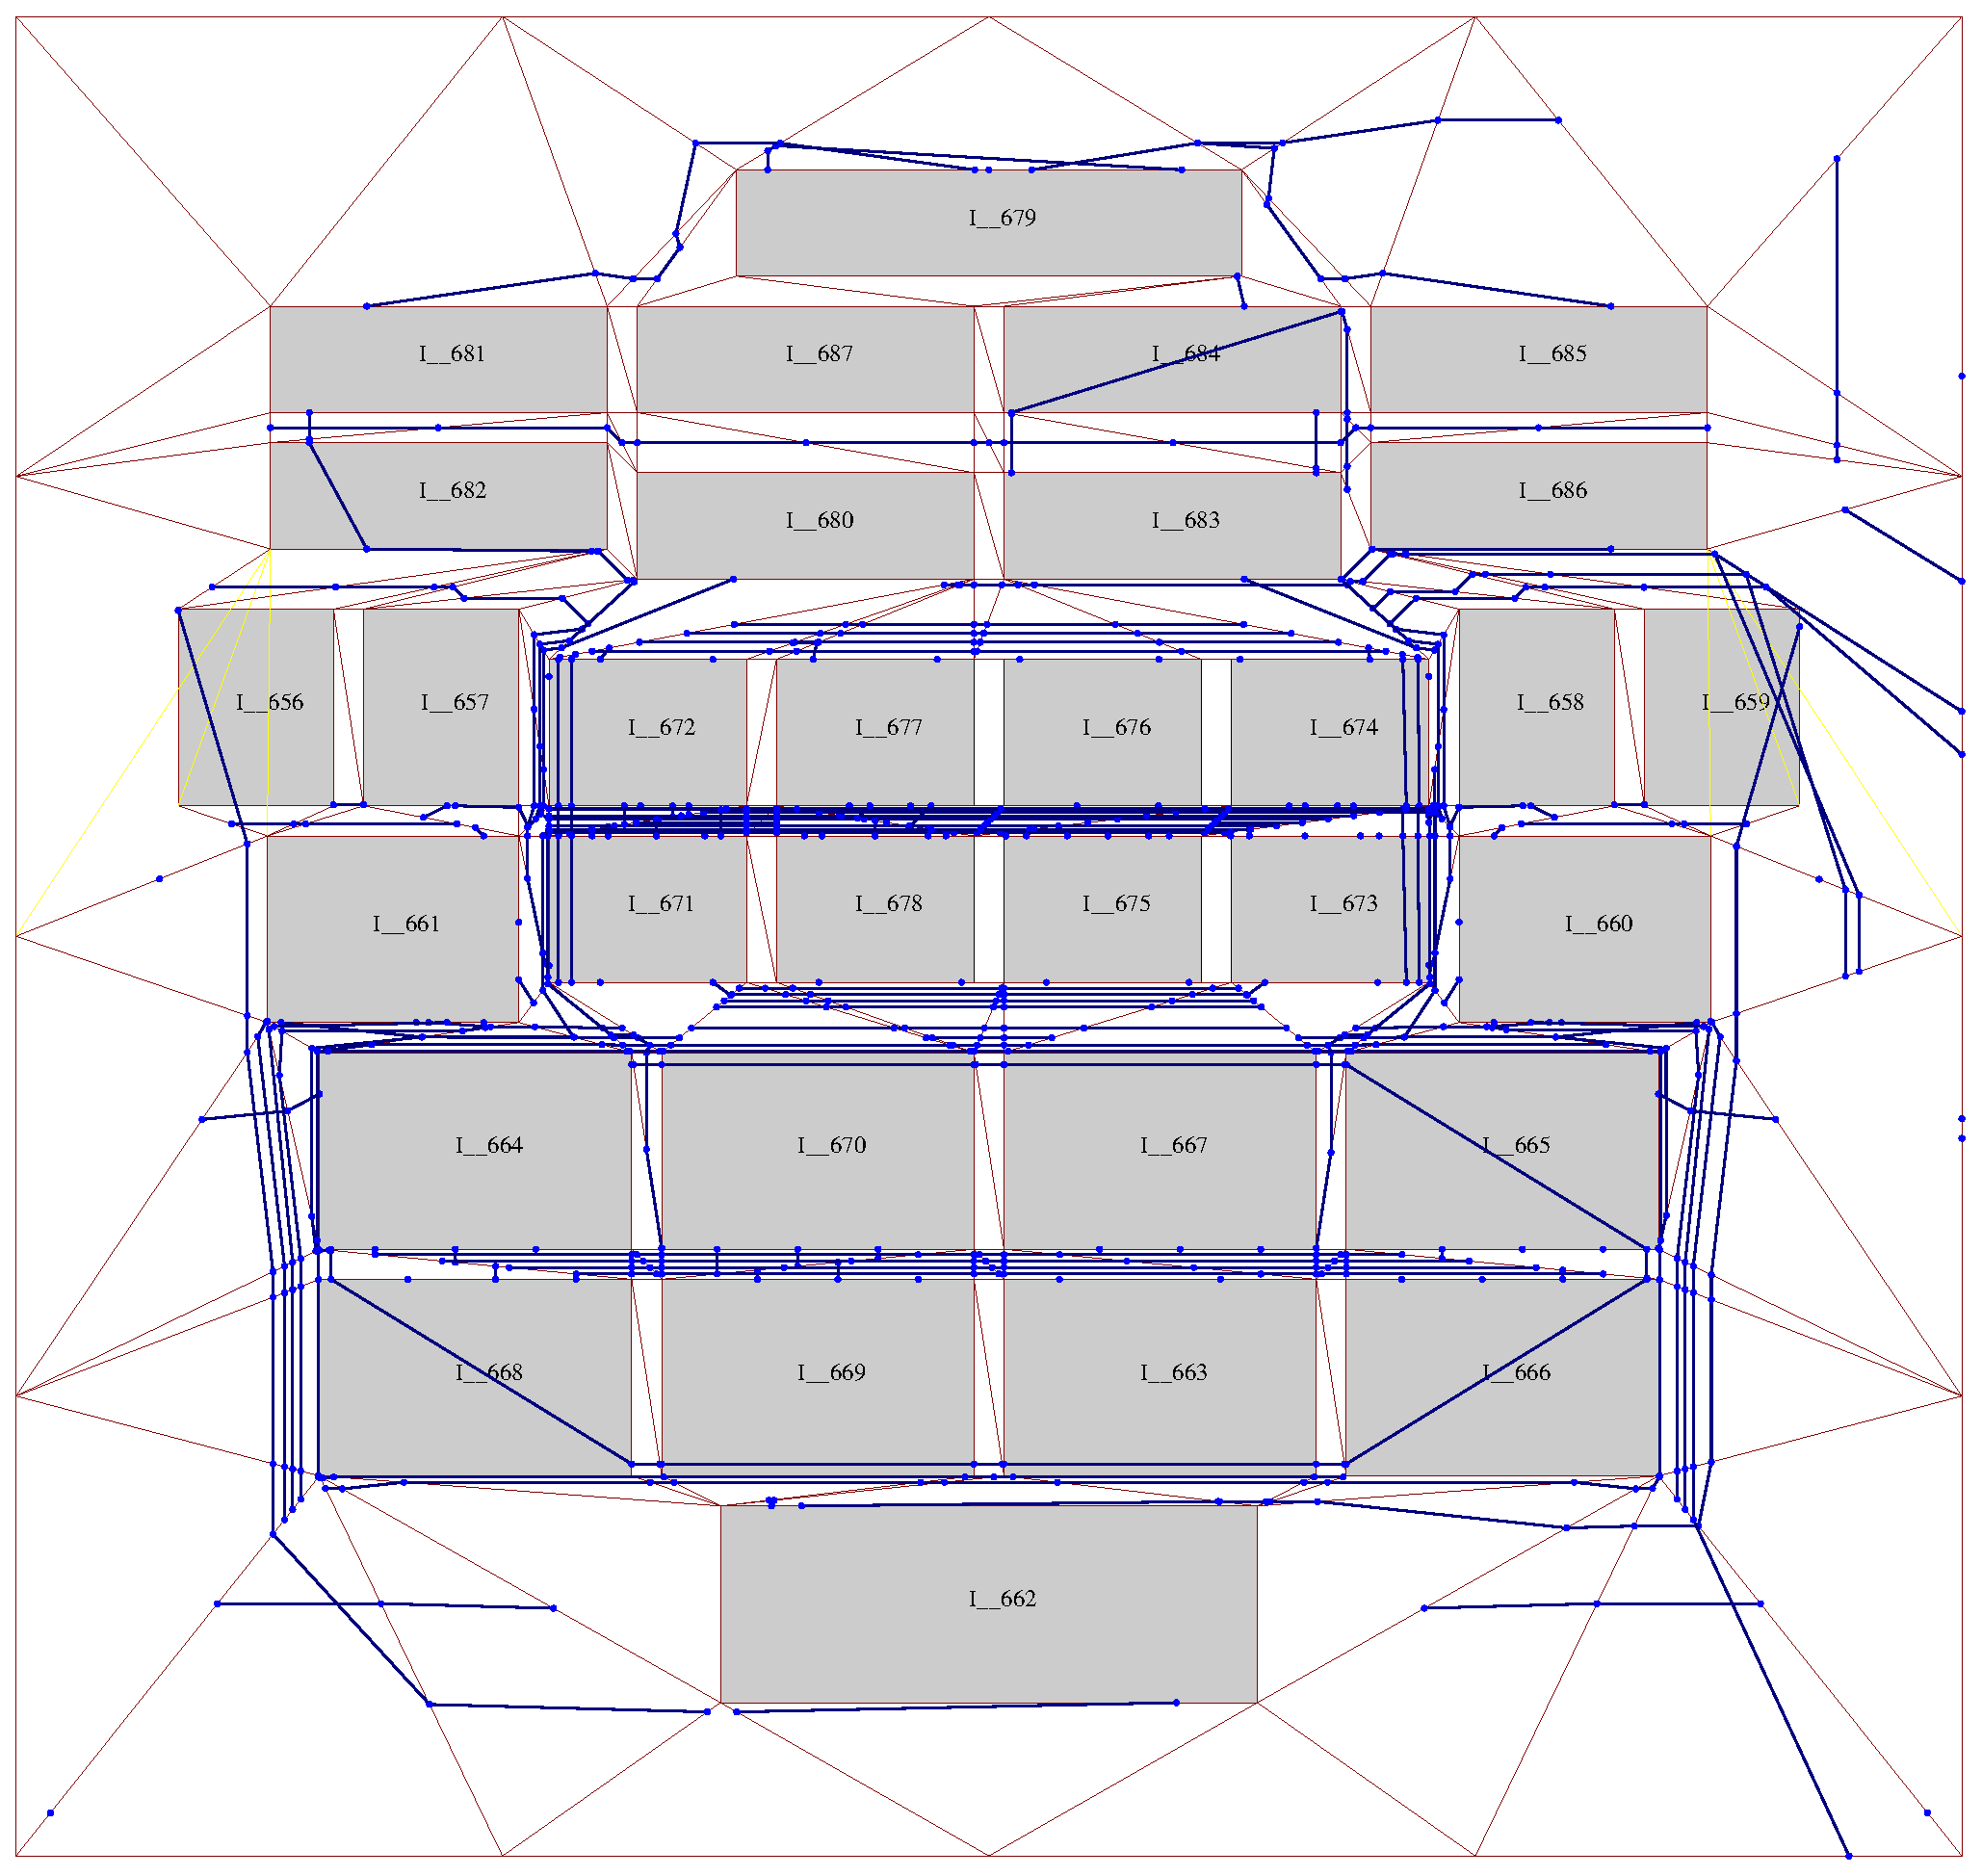
\includegraphics[width=\textwidth]{Fig/VGAProto.eps}
          \caption{VGA umc65nm}\label{fig:VGAProto}
          \end{subfigure}
        \caption{Illustration of crossing graph for OpAmp and VGA before and after updating: (a) extracted crossing graph of OpAmp under umc90nm (b)updated crossing graph under tsmc90nm (c) extracted crossing graph of OpAmp under umc90nm. (d) updated crossing graph of VGA under umc65nm}
        \label{fig:CDTResult}
      \end{figure}

    

    In the third experiment, we further practice original topology with CDT-based migrated routing and our approach on a large multi-level design in Section~\ref{subsec:ExpLDO}. 
    All the experimental results have passed layout verification via DRC, LVS checks, and the simulation data is listed in Table~\ref{table:MigrationPerf}, Table~\ref{table:MultProto} and Table~\ref{table:HierProto}.

    \subsection{Placement in Original Topology with Different Routing Migrations}\label{sec:ExpMigration}


      First of all, we focus on migrating two circuits based on umc90nm technology to other technology nodes which are umc65nm and tsmc90nm. To reach the requirement of design migration, one circuit should be re-generated on the target technology for the same functionality while satisfying the performance specification. 

      
      
      \begin{sidewaystable}[ht]
        \hspace{-1em}
        \begin{threeparttable}
        \scriptsize
        \begin{center}
          \caption{Routing Completeness and Performance Comparisons among Migration Targets}\label{table:MigrationPerf}
        \begin{tabular}{|c|c|c|c|c|c|c|c|c|c|c|c|c|}
          \toprule  
          \hline
            \multirow{2}{*}{Circuit}& 
            \multirow{2}{*}{Layout} & 
            \multicolumn{2}{c|}{Overall Routing \tnote{a}} & 
            \multicolumn{2}{c|}{Auto Routing \tnote{b}} & 
            \multicolumn{2}{c|}{Routing Com.\tnote{c} (\%)} & 
            \multirow{2}{1cm}{$A_v$ ($dB$)} & 
            \multirow{2}{1cm}{BW ($MHz$)} & 
            \multirow{2}{1cm}{PM ($deg$)} & 
            \multirow{2}{1cm}{Power ($\mu W$)}  &
            \multirow{2}{*}{Time }\\
            \cline{3-8} 
            & & WL ($\mu m$) & WS \# &  WL ($\mu m$) & WS \#  &  WL ($\mu m$) & WS \# & & & & & \\
          \hline
          OpAmp:umc90nm &  Origin & 351.438 & & - &-  &-& - & 48.653 &  110.9 & 45.882  & 120.34 &  8 hrs \\
          \hline
          OpAmp:umc65nm &  \cite{msc-bhattacharya-tcad06}+RtMaMi &  321.44 & 38 & - & - & - & - & 43.421& 110.4 &53.294 & 118.66 &  8 hrs \\
          \hline
          OpAmp:umc65nm & \cite{msc-bhattacharya-tcad06}+RtNoMi& 414.84 & 45 & 312.471 & 31 & 75.3\% & 68.89\%& 43.02& 108.6& 56.6& 118.36 &  100 mins \\
          \hline
          OpAmp:umc65nm &  Ours & 298.99& 40 & 231.15 &32 &  77.3 \%& 80.00\% & 43.36 & 110.4 & 56.6 & 118.69 & 40 mins \\
          \hline
          OpAmp:tsmc90nm  &  Ours & 286.954& 38 &  215.204& 33&  74.99 \% & 86.84\%& 45.0 &117.0 &55.9 & 113.3 & 40 mins \\
          \hline
          VGA:umc90nm & Origin &  3628.25  &  281& -&-&- & - & 18.48 & 7.237&86.645 & 596.74 & 2 days \\
          \hline
          VGA:umc65nm & \cite{msc-bhattacharya-tcad06}+RtMaMi &  3011.83& 283 & -& - &- & - & 18.57 & 7.427 &90.75& 566.81&   2 days \\
          \hline
          VGA:umc65nm & Ours & 3385.849& 266 &  2877.99& 238 & 85 \% & 89.47\%&18.68 & 7.41& 89.3 & 569.1& 553 mins  \\
          \hline
        \end{tabular}
        \begin{tablenotes}
          \item [a] Overall routing characteristics including the wirelength and the number of wire segments. 
          \item [b] Automatic generated routing characteristics
          \item [c] Routing completeness is the ratio between auto-gen routing and overall routing. 
        \end{tablenotes}
        \end{center}
        \end{threeparttable}
      \end{sidewaystable} 
         

      Figure~\ref{fig:CDTResult} illustrates the crossing graph generated from template layouts and the updated graph from target layouts. Figure~\ref{fig:OrigOpamp} shows the crossing graph of OpAmp with only one routing path being displayed, and Figure~\ref{fig:OpampProto} shows the updated crossing graph for tsmc90nm. We can find out that the routing behavior is recorded by the graph when the placement is changed. Figure~\ref{fig:OrigVGA} shows one of the crossing graphs of VGA circuit since VGA has more than one hierarchy with all routing paths on it. Figure~\ref{fig:VGAProto} shows the updating graph for umc65nm. Although VGA has much more routing nets than OpAmp, routing behavior of each routing paths is preserved in the crossing graph. The purple points along the routing edges implies the original vertices of wire segments, which are not regarded as crossing vertices, and the blue points are crossing points as mentioned in Section~\ref{sec:CGC}. Figure~\ref{fig:PPL_OPT90} and Figure~\ref{fig:PPL_VGAU65} illustrate the updated crossing graphs of Figure~\ref{fig:ML_OPU90} and Figure~\ref{fig:ML_VGAU90} respectively. The yellow edges are the {\it invalid} crossing edges, after updating. As mentioned in Section~\ref{sec:updateG}, these {\it invalid} crossing edges overlap the blocks after updating.

      \begin{figure}[ht]
        \centering
          \begin{subfigure}[t]{0.4\textwidth}
          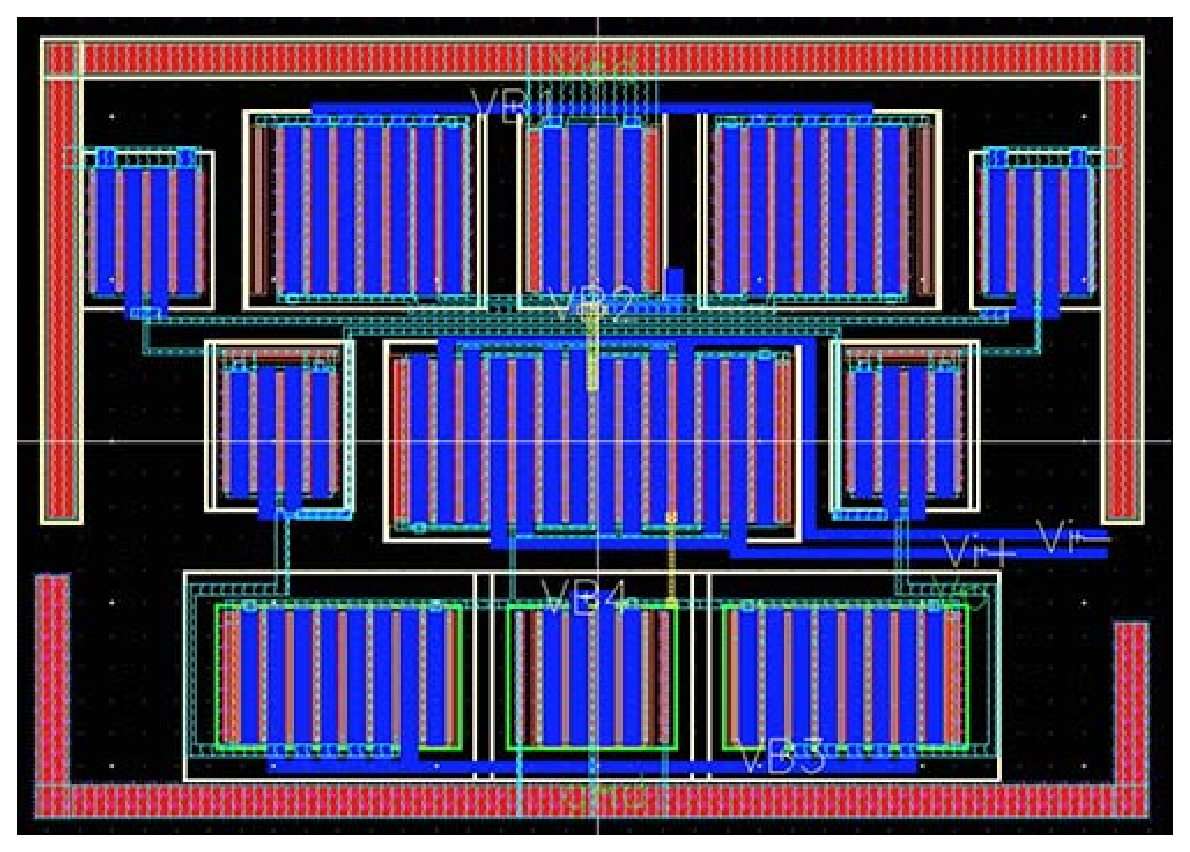
\includegraphics[width=\textwidth]{Fig/ML_OPU90.eps}
          \caption{OpAmp:umc90nm Ori. Layout}\label{fig:ML_OPU90}
          \end{subfigure}
          \begin{subfigure}[t]{0.4\textwidth}
          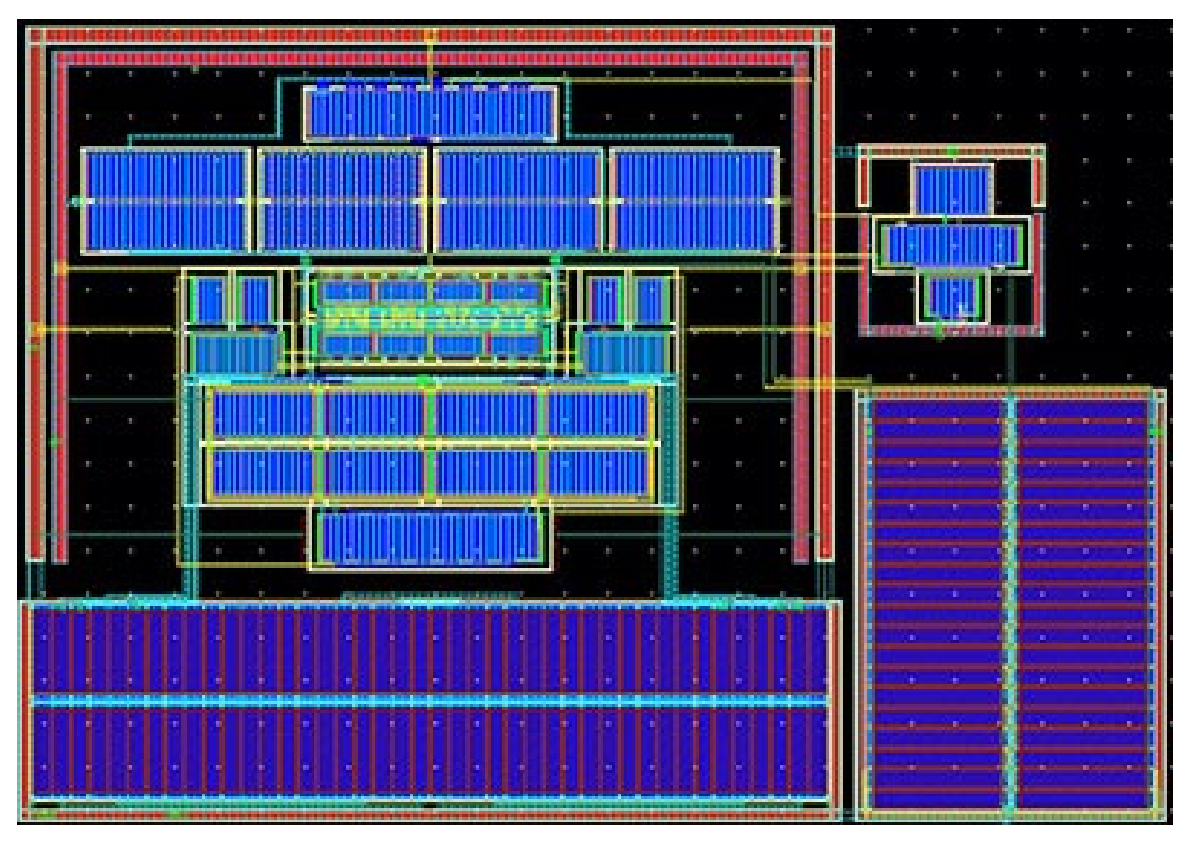
\includegraphics[width=\textwidth]{Fig/ML_VGAU90.eps}
          \caption{VGA:umc90nm Ori. Layout}\label{fig:ML_VGAU90}
          \end{subfigure}
          \begin{subfigure}[t]{0.4\textwidth}
          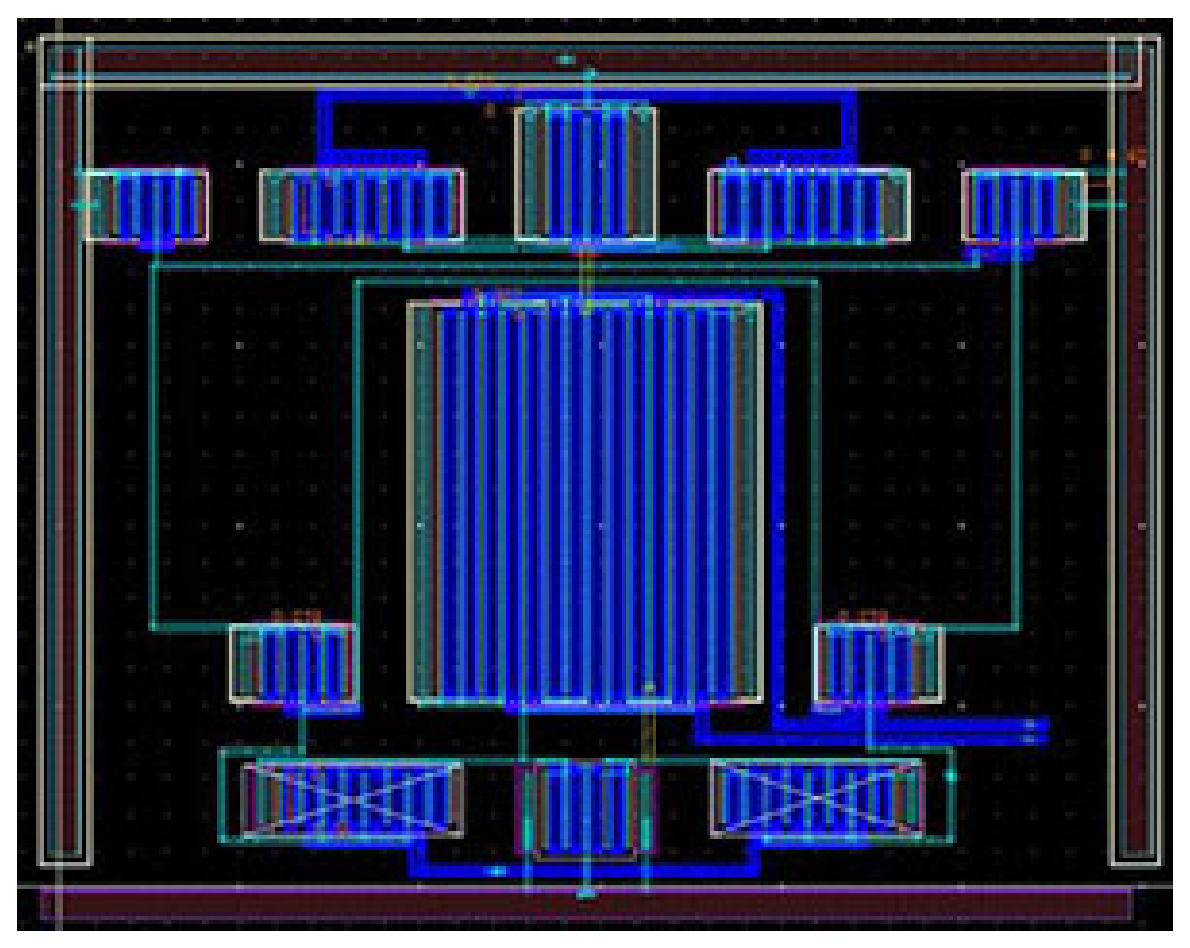
\includegraphics[width=\textwidth]{Fig/PPL_OPT90.eps}
          \caption{OpAmp:tsmc90nm our approach}\label{fig:PPL_OPT90}
          \end{subfigure}
          \begin{subfigure}[t]{0.4\textwidth}
          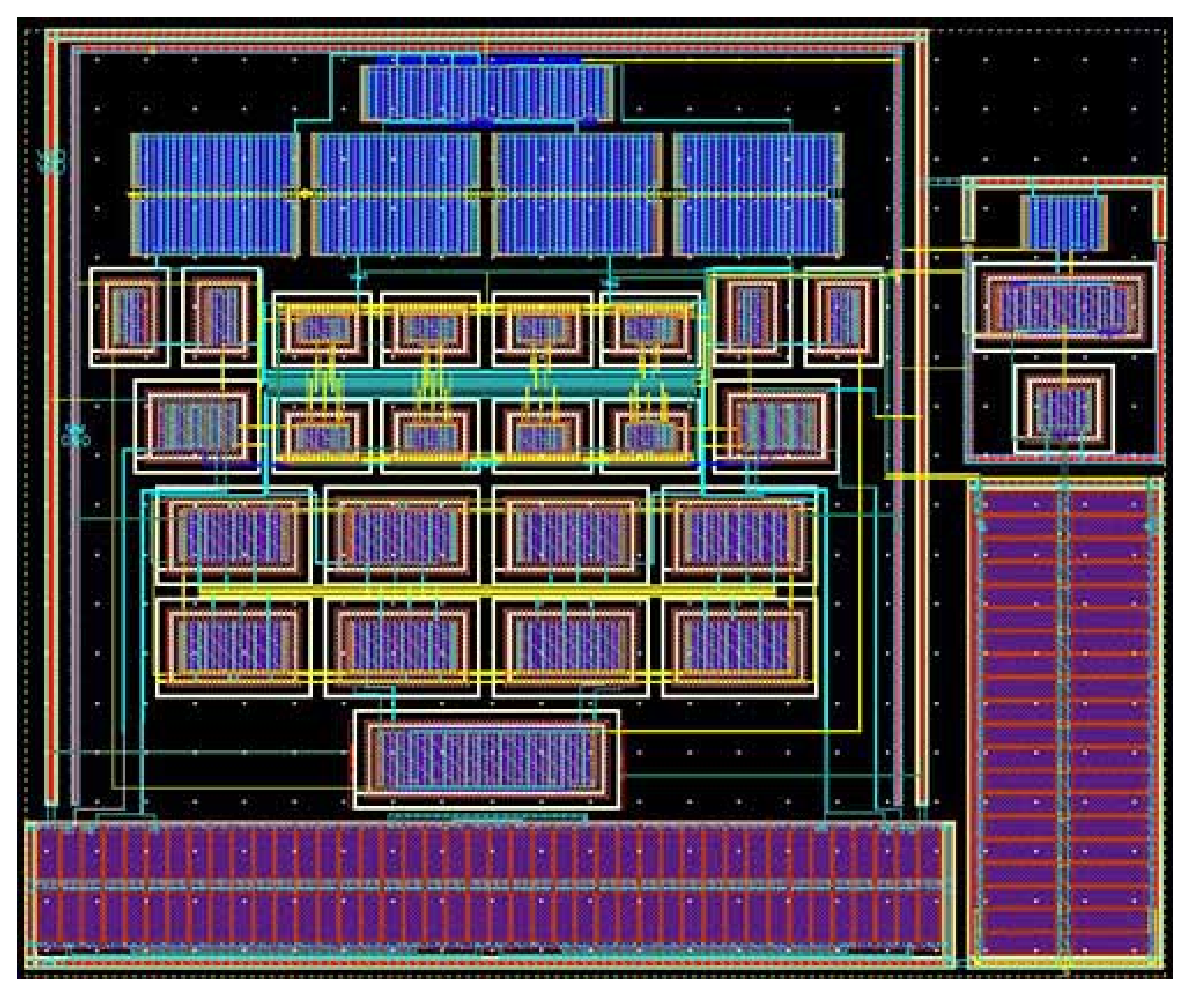
\includegraphics[width=\textwidth]{Fig/PPL_VGAU65.eps}
          \caption{VGA:umc65nm our approach}\label{fig:PPL_VGAU65}
          \end{subfigure}
        \caption{Migration comparison on Op-Amp design among (a) Original layout. (b) Placement fully and routing fully migrated to umc65nm (c) Placement with original topology and routing preserved to umc65nm and (d) Placement with original topology and routing preserved to tsmc90nm.}\label{fig:Layout}
      \end{figure}



      Figure~\ref{fig:Layout} illustrates the layout results of migrated designs. Figure~\ref{fig:ML_OPU90} and Figure~\ref{fig:ML_VGAU90} illustrates the original layouts of OpAmp and VGA respectively. Figure~\ref{fig:PPL_OPT90} gives the migrated results obtained by our methodology under tsmc90nm technology. It is easy to observe that even though placement is changed due to different block size, the routing correlation with placement is preserved under tsmc90nm technology. Figure~\ref{fig:PPL_VGAU65} illustrates the migrated VGA under umc65nm. Since there are three common-centroid structures in the VGA layout, more wires are connected inside these common-centroid structures. While RtMaMi takes time to re-construct the routing in manual, the crossing graph can migrate the relative location for these wires in a flexible manner.


      Based on migrated placement by \cite{msc-bhattacharya-tcad06} and our approach, there are three migration strategies performed towards OpAmp and VGA design under different technologies. These are RtMaMi, RtNoMi and our approach. Table~\ref{table:MigrationPerf} records the wirelength, the number of wire segments and the simulation data. We compare the overall routing WL, automatically generated WL and the routing completeness on wirelength firstly. The overall wirelength consists of wires by manual automated routing. Since circuit sizing in umc65nm can be scaled down to satisfy performance specifications, the devices' size and WL are proportionally smaller as well. The routing completeness of WL is expressed as the ratio between auto-generated routing over total wirelength. However, the distance between blocks are diverse to measure the routing completeness with wirelength is not comprehensive. Therefore, we also consider the re-coverage of wire segment (WS). The routing completeness of WS implies how many essential wire segments is automatically generated by program. Obviously, even though RtNoMi generates routing result automatically, it still takes time to refine the layout for accuracy. We can see the routing completeness of RtNoMi are 75.3\% and 68.9\% for WL and WS respectively. We can tell that, most of the RtNoMi results in the OpAmp circuit are failed with LVS checking so that it leaves part of wire in manual refinement.

      \begin{figure}[ht]
        \centering
        \begin{subfigure}[t]{0.2\textwidth}
        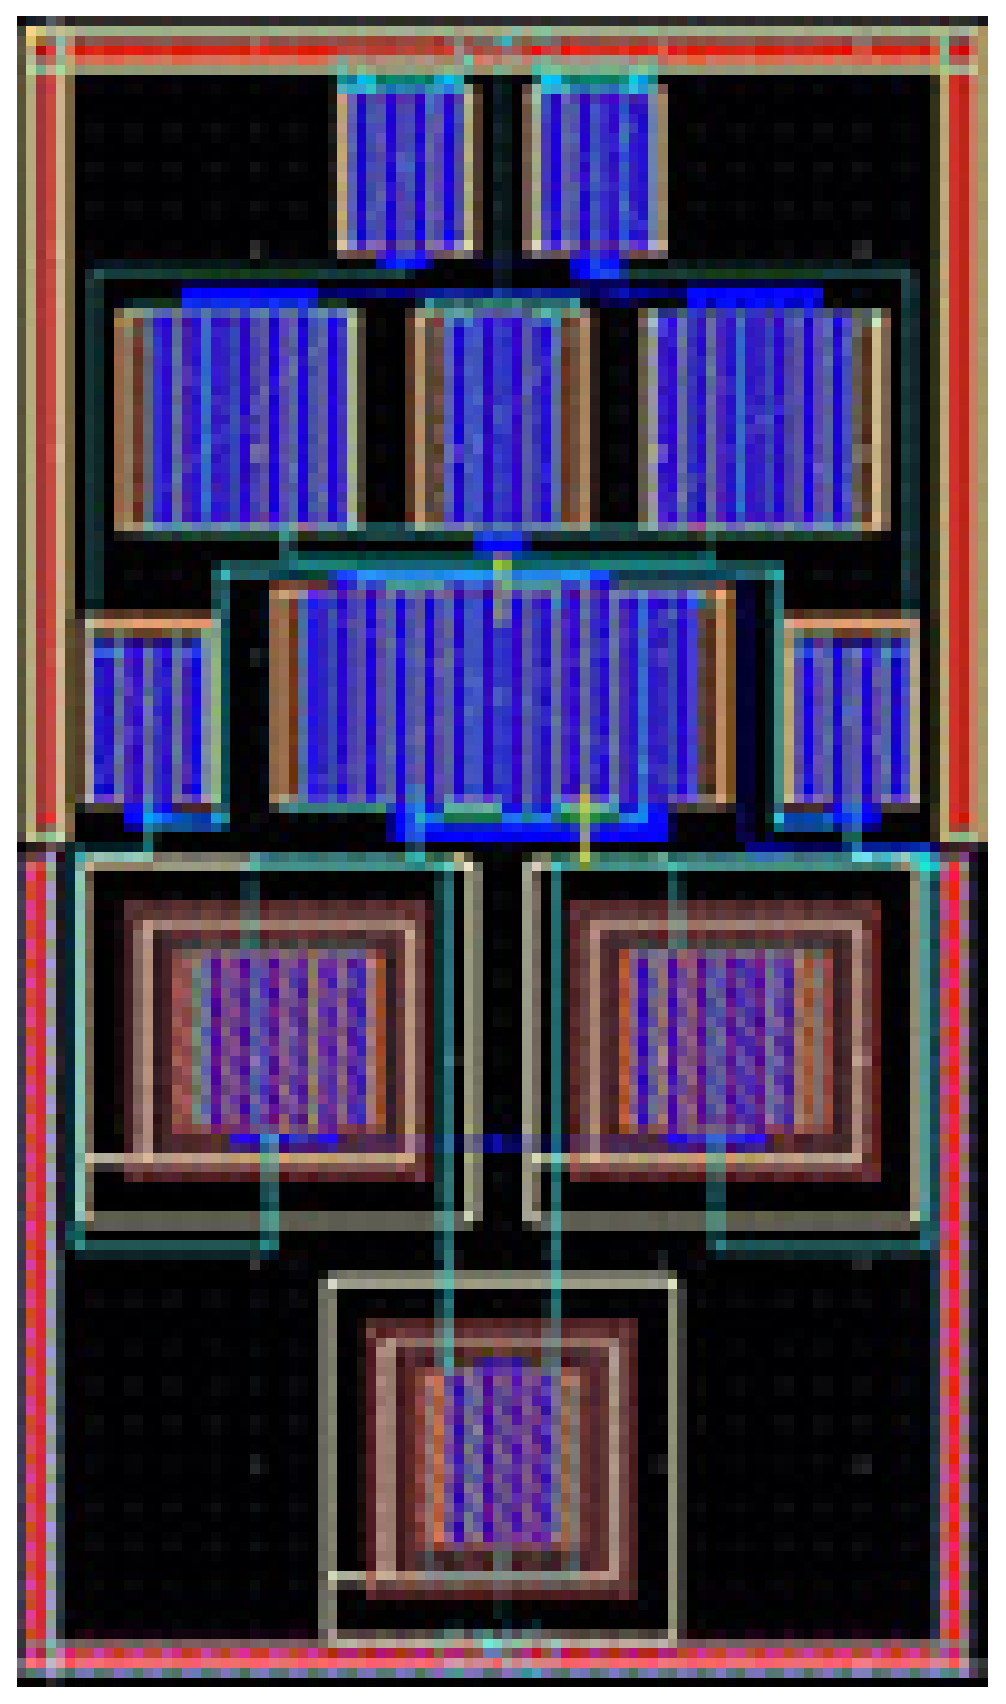
\includegraphics[width=\textwidth]{Fig/MultTopo_Topo2.eps}
        \caption{Topo2}\label{fig:Topo2}
        \end{subfigure}
        \begin{subfigure}[t]{0.2\textwidth}
        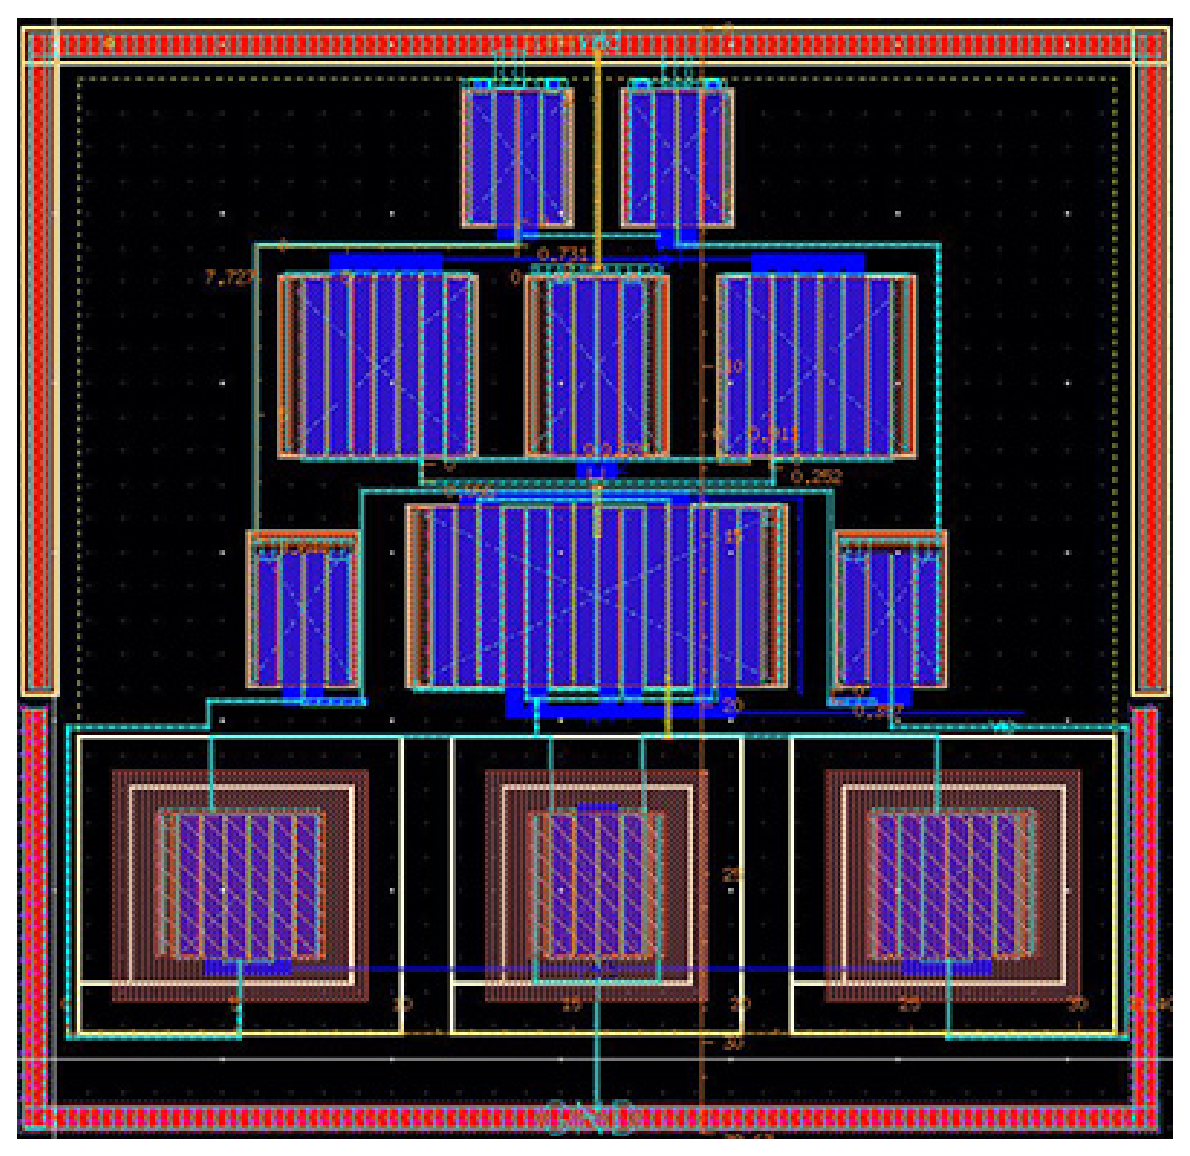
\includegraphics[width=\textwidth]{Fig/MultTopo_Topo3.eps}
        \caption{Topo3}\label{fig:Topo3}
        \end{subfigure}
        \begin{subfigure}[t]{0.2\textwidth}
        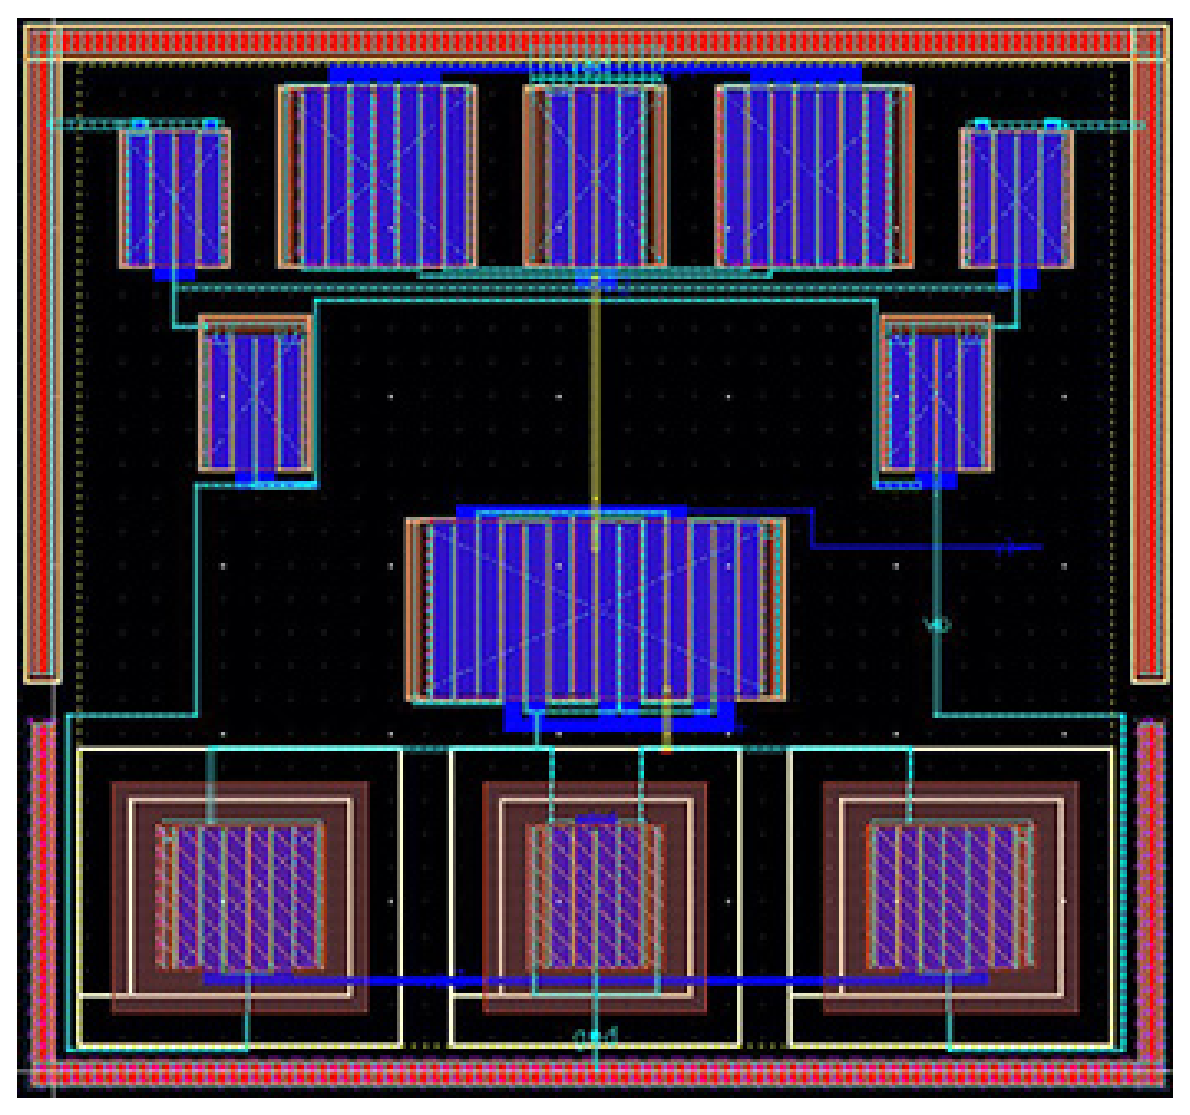
\includegraphics[width=\textwidth]{Fig/MultTopo_Topo4.eps}
        \caption{Topo4}\label{fig:Topo4}
        \end{subfigure}
        \begin{subfigure}[t]{0.2\textwidth}
        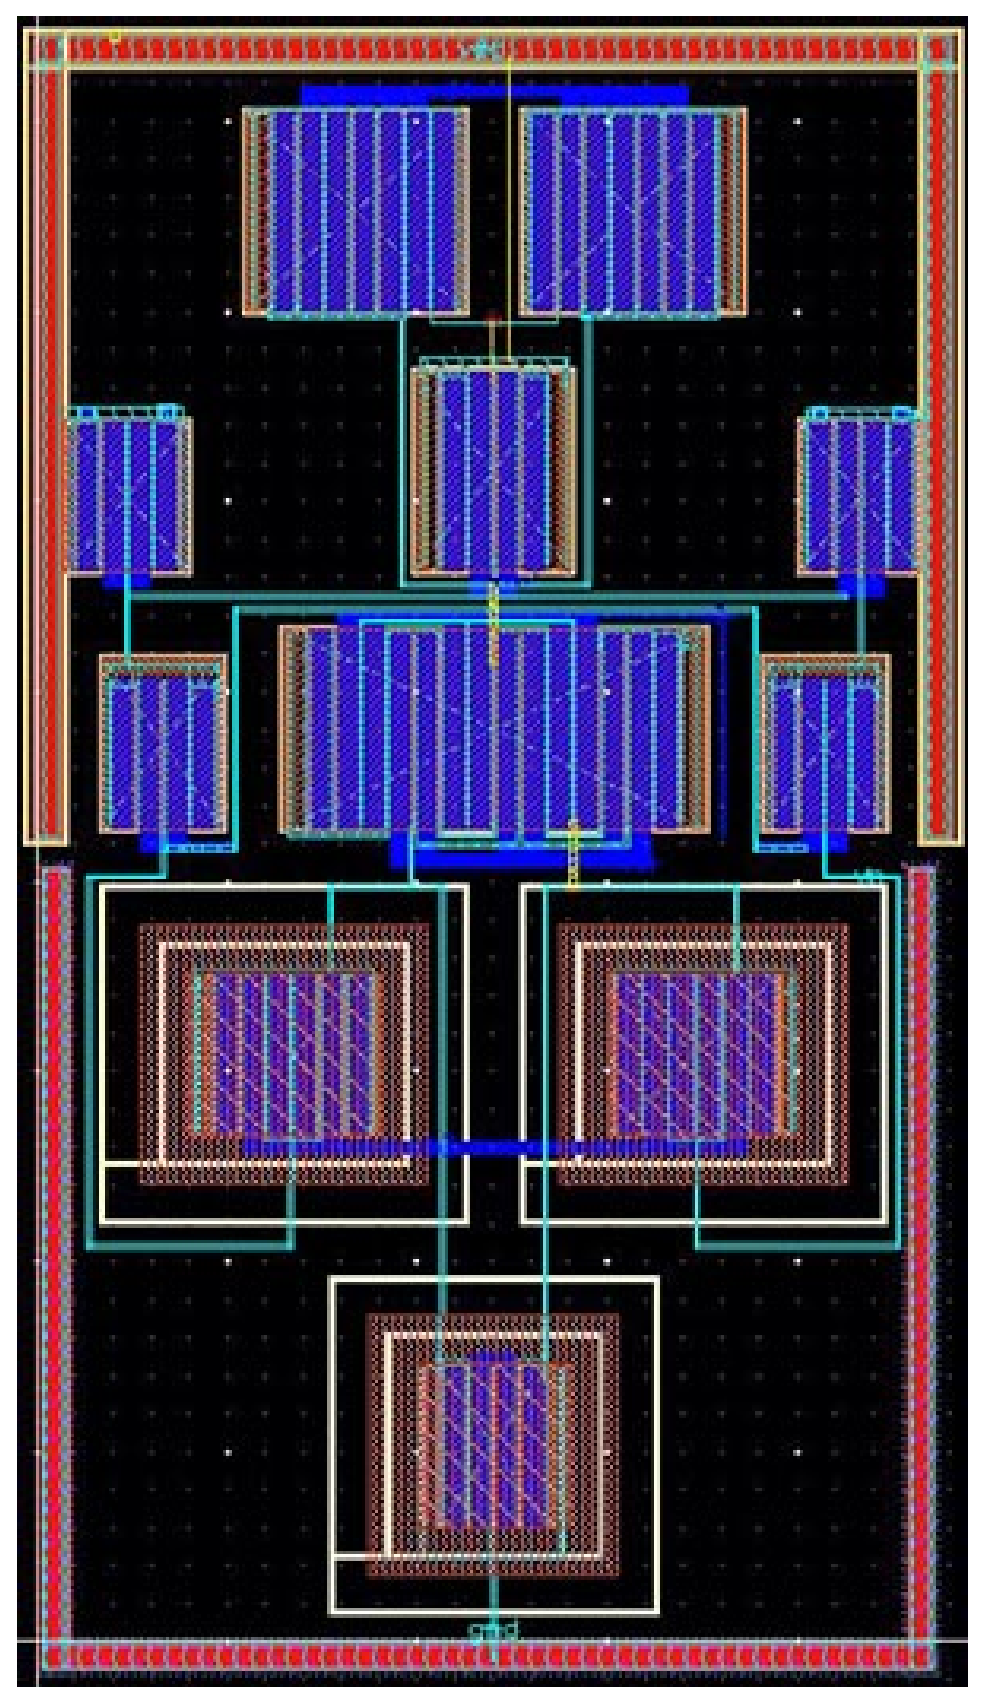
\includegraphics[width=\textwidth]{Fig/MultTopo_Topo5.eps}
        \caption{Topo5}\label{fig:Topo5}
        \end{subfigure}
        \begin{subfigure}[t]{0.2\textwidth}
        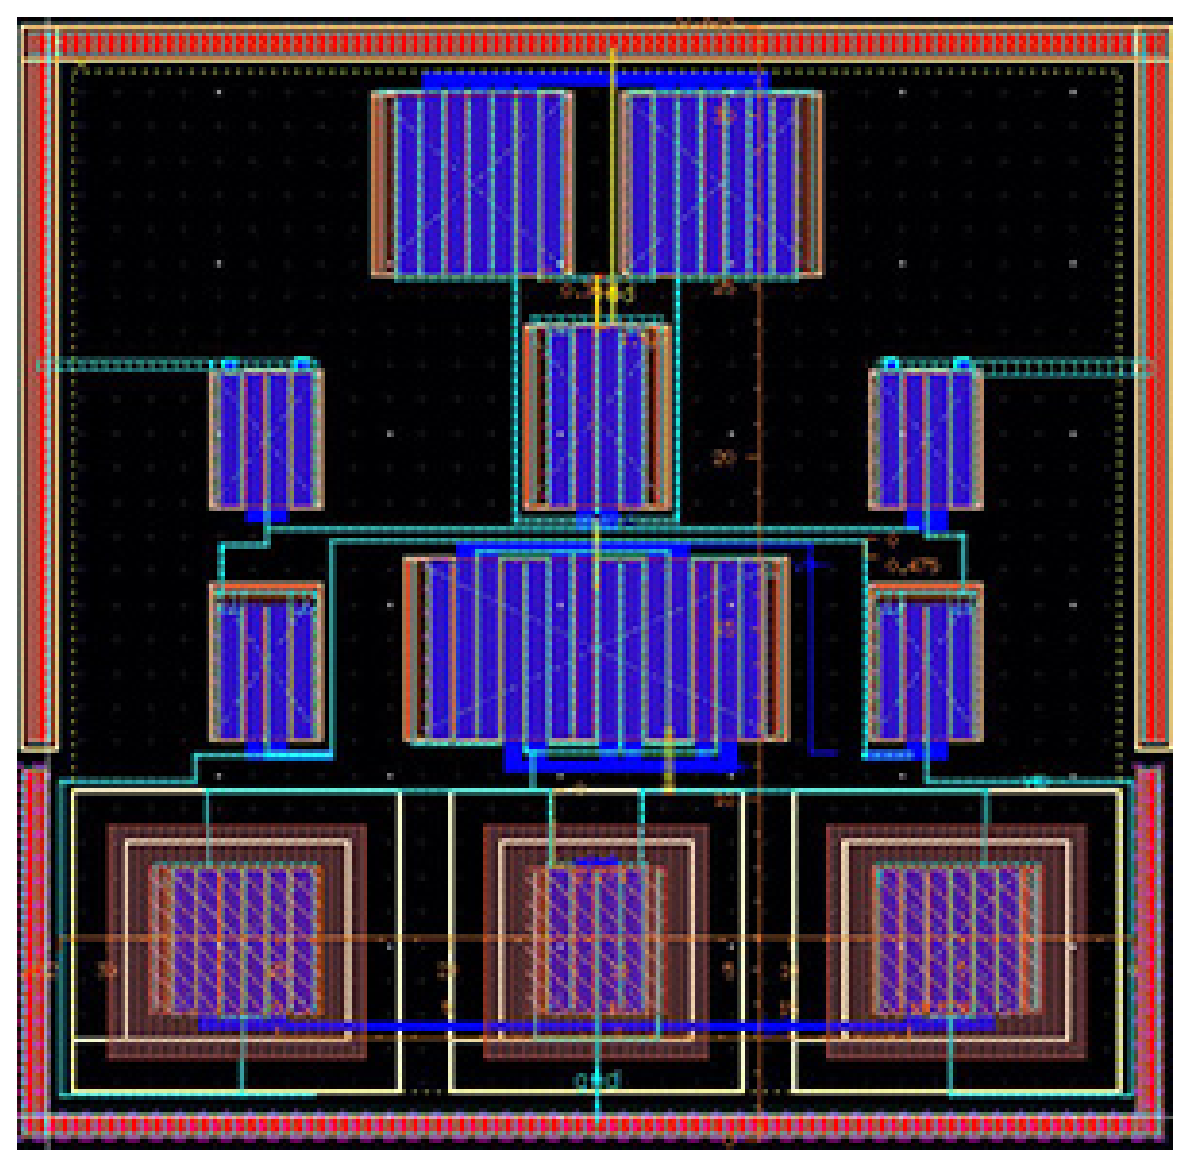
\includegraphics[width=\textwidth]{Fig/MultTopo_Topo6.eps}
        \caption{Topo6}\label{fig:Topo6}
        \end{subfigure}
        \begin{subfigure}[t]{0.2\textwidth}
        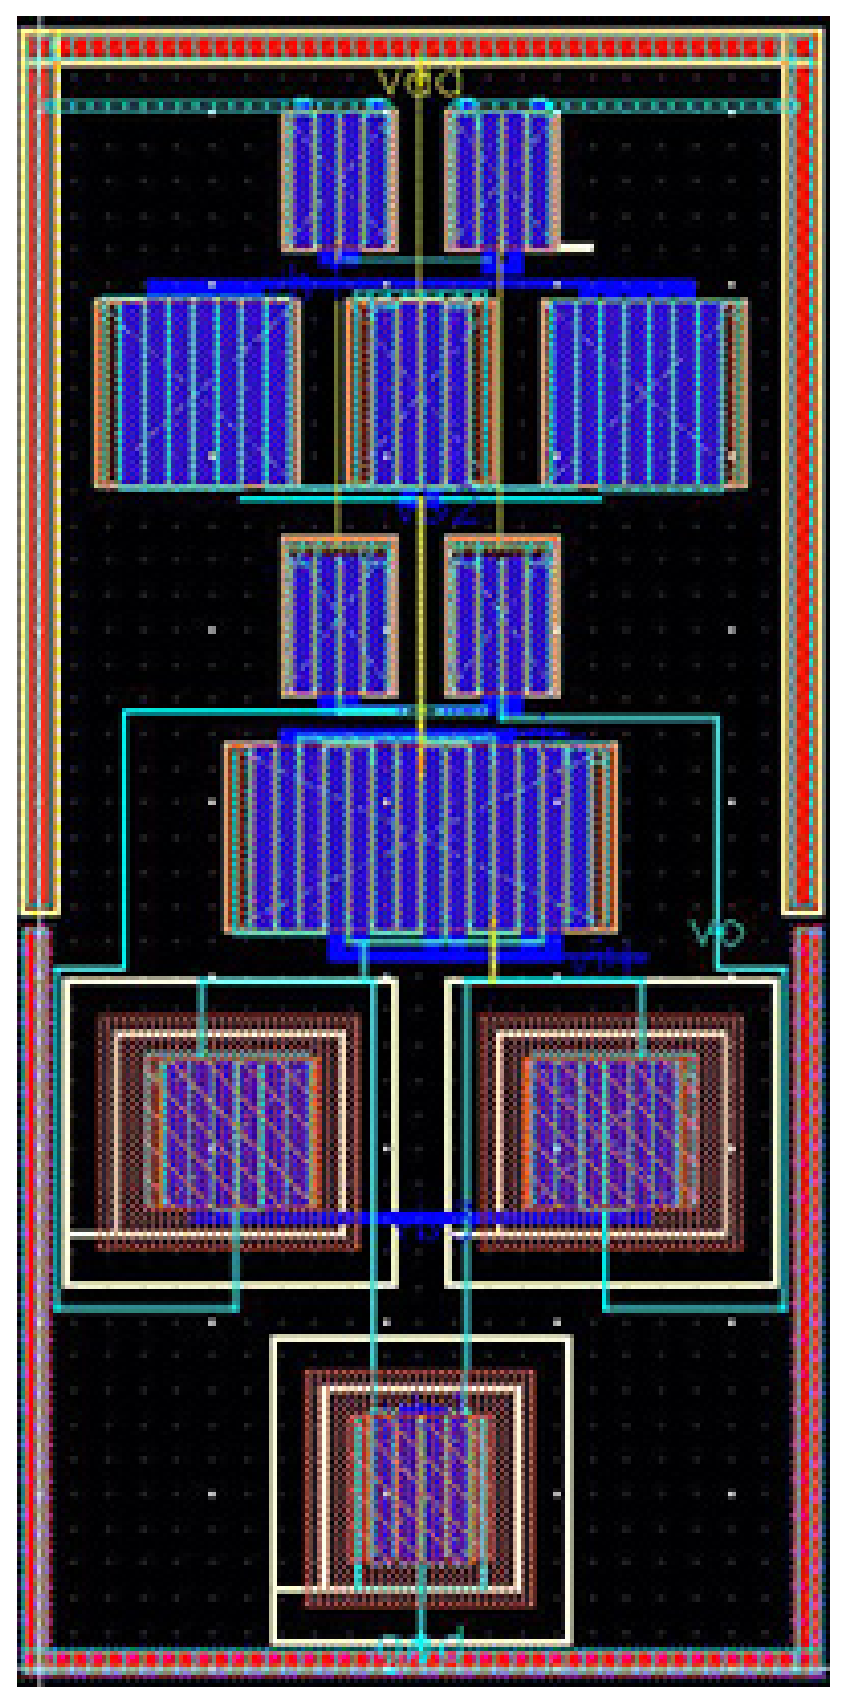
\includegraphics[width=\textwidth]{Fig/MultTopo_Topo7.eps}
        \caption{Topo7}\label{fig:Topo7}
        \end{subfigure}
        \begin{subfigure}[t]{0.2\textwidth}
        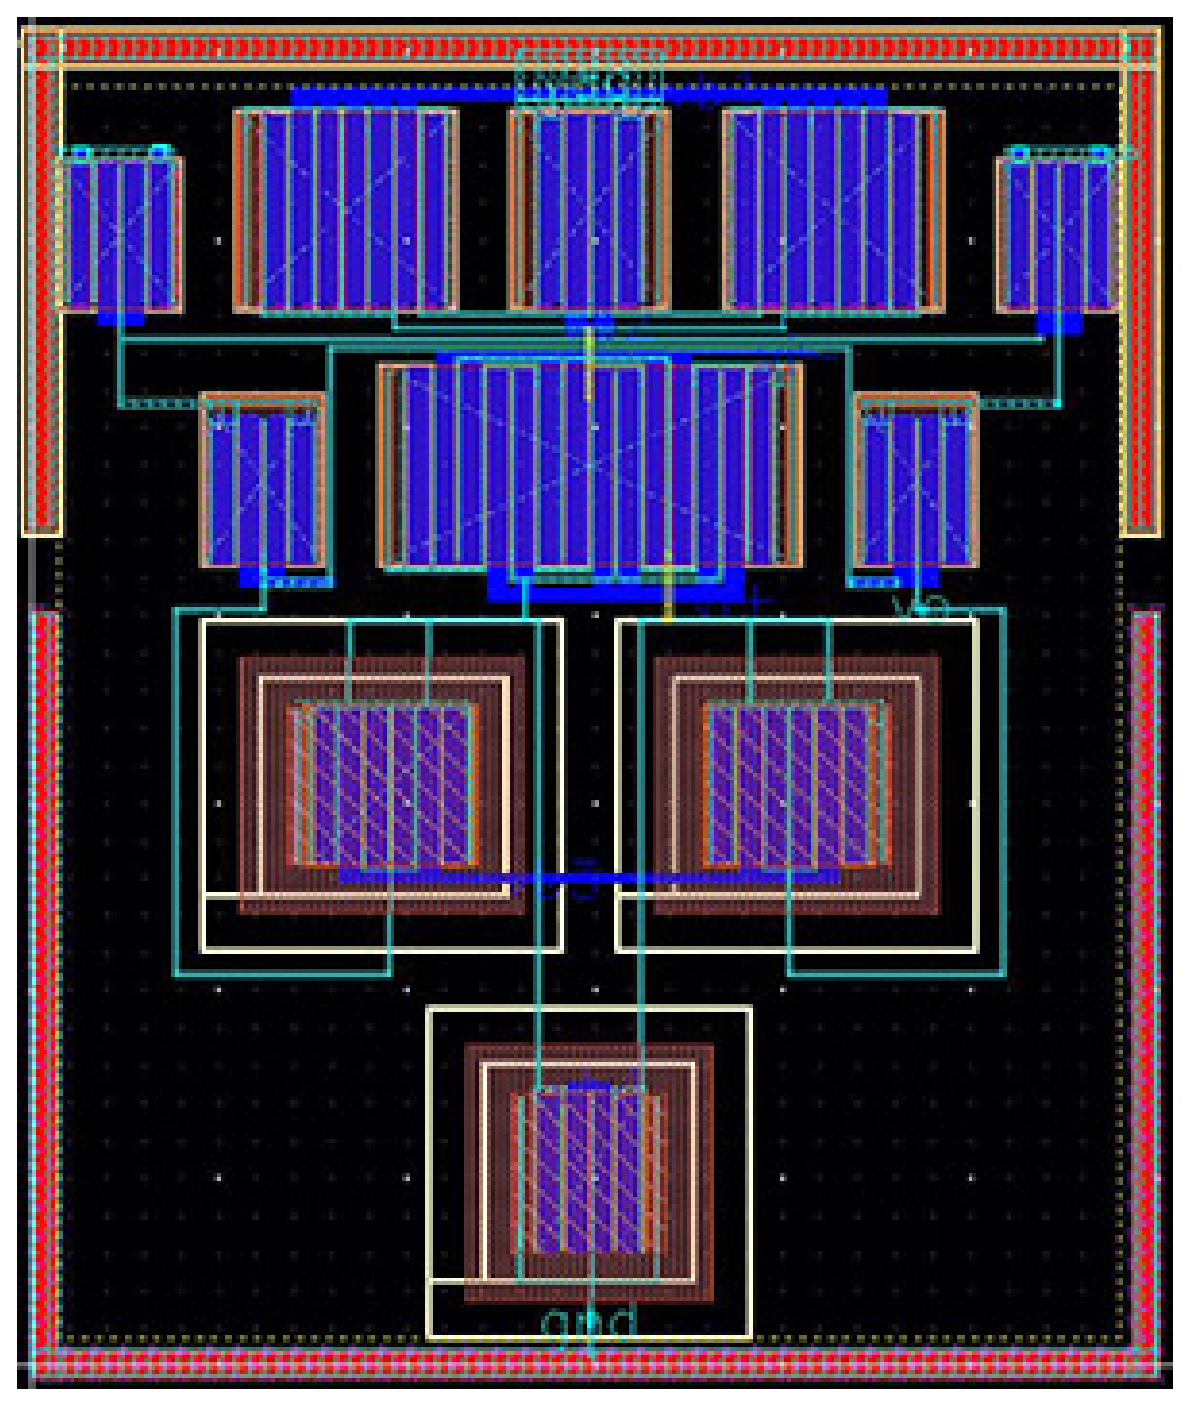
\includegraphics[width=\textwidth]{Fig/MultTopo_Topo8.eps}
        \caption{Topo8}\label{fig:Topo8}
        \end{subfigure}
        \caption{Multiple prototype of layouts achieved by our approach with 7 topologies respectively.}
        \label{fig:MultTopo}
      \end{figure}

      \begin{sidewaystable}
        \scriptsize
        \begin{center}
          \caption{Routing Completeness and Performance Comparisons among Multiple Migrated Placements}\label{table:MultProto}
          \begin{tabular}{|c|c|c|c|c|c|c|c|c|c|c|c|}
            \toprule
            \hline
            \multirow{2}{*}{Placement}& 
            \multirow{2}{*}{Routing} & 
            \multicolumn{2}{c|}{Overall Routing}  & 
            \multicolumn{2}{c|}{Auto Routing } & 
            \multicolumn{2}{c|}{Routing Com. (\%)} & 
            \multirow{2}{1cm}{\scriptsize $A_v$/$A_v^{WSR}$ ($dB$)} & 
            \multirow{2}{1.3cm}{\tiny $BW$/$BW^{WSR}$ ($MHz$)} & 
            \multirow{2}{1.3cm}{\tiny $PM$/$PM^{WSR}$ ($deg$)} & 
            \multirow{2}{*}{Time}\\
            \cline{3-8} 
            & & WL ($\mu m$) & WS \#  &  WL ($\mu m$) & WS \# &  WL & WS \# & & & & \\
            \hline
              Original Topo. & \multirow{8}{*}{RtMaMi} & 321.44 & 38 &\multirow{8}{*}{-} & \multirow{8}{*}{-} & \multirow{8}{*}{-} & \multirow{8}{*}{-} & 43.421/- & 110.4/- & 53.29/- & 8 hrs \\ \cline{1-1} \cline{3-4} \cline{9-12}
              \cite{ALP_YPWeng_iccad2011}:Topo2 & & 210.53 & 34 & & & & & 43.398/- & 111.22/- & 53.723/- & 3 hrs \\ 
              \cite{ALP_YPWeng_iccad2011}:Topo3 & & 203.2 & 33 & & & & & 43.398/- & 110.63/- & 53.601/- & 3 hrs \\ 
              \cite{ALP_YPWeng_iccad2011}:Topo4 & & 206.625 & 34 & & & & & 43.41/- & 111/- & 53.669/- & 3 hrs \\ 
              \cite{ALP_YPWeng_iccad2011}:Topo5 & & 228.519 & 39 & & & & & 43.393/- & 111/- & 53.617/- & 3 hrs \\ 
              \cite{ALP_YPWeng_iccad2011}:Topo6 & & 274.525 & 38 & & & & & 43.393/- & 110.56/- & 53.496/- & 3 hrs \\ 
              \cite{ALP_YPWeng_iccad2011}:Topo7 & & 226.495 & 32 & & & & & 43.398/- & 111.59/- & 53.917/- & 3 hrs \\ 
              \cite{ALP_YPWeng_iccad2011}:Topo8 & & 238.28 & 36 & & & & & 43.422/- & 110.98/- & 53.412/- & 3 hrs \\
            \hline
              Original Topo. & \multirow{8}{*}{RtNoMi} & 414.84 & 45 & 312.471 & 31 & 75.3\% & 68.89\% & 43.02/- & 108.6/- & 56.6/- & 100 mins \\ \cline{1-1} \cline{3-12}
              \cite{ALP_YPWeng_iccad2011}:Topo2 & & 401.896 & 48 & 316.8 & 37 & 78.8\% & 77.08\% & 42.69/- & 112.8/- & 57.57/- & 60 mins \\
              \cite{ALP_YPWeng_iccad2011}:Topo3 & & 392.777 & 45 & 311.2 & 35 & 79.23\% & 77.78\% & 42.99/- & 109.3/- & 57.35/- & 40 mins \\
              \cite{ALP_YPWeng_iccad2011}:Topo4 & & 486.795 & 47 & 369.3 & 34 & 78.86\% & 72.34\% & 43.03/- & 108.2/- & 57.3/- & 35 mins \\
              \cite{ALP_YPWeng_iccad2011}:Topo5 & & 395.9 & 44 & 316.6 & 36 & 79.97\% & 81.82\% & 42.74/- & 108.6/- & 57.71/- & 1 hrs \\
              \cite{ALP_YPWeng_iccad2011}:Topo6 & & 408.7 & 46 & 316.8 & 34 & 77.51\% & 73.91\% & 42.75/- & 108.8/- & 57.34/- & 65 mins\\
              \cite{ALP_YPWeng_iccad2011}:Topo7 & & 406.55 & 44 & 298.1 & 32 & 73.32\% & 72.73\% & 42.98/- & 109.6/- & 57.7/- & 43 mins \\
              \cite{ALP_YPWeng_iccad2011}:Topo8 & & 435.56 & 41 & 334.7 & 33 & 76.84\% & 80.49\% & 42.77/- & 108.7/- & 57.54/- & 45 mins \\
            \hline
              Original Topo. & \multirow{8}{*}{Ours} & 298.99 & 40 & 231.15 & 32 & 77.31\% & 80\% & 43.348/43.36 & 110.37/110.4 & 56.6/56.6 & 42 mins \\ \cline{1-1} \cline{3-12}
              Ours:Topo2 & & 275.569 & 38 & 204.176 & 31 & 79.27\% & 81.58\% & 43.388/43.42 & 109.6/109.0 & 49.3/50.7  &  41 mins \\
              Ours:Topo3 & & 278.023 & 43 & 232.866 & 35 & 83.7\% & 81.4\% &  43.41/43.431 & 109.8/110.2 & 55.6/55.6 & 31 mins \\
              Ours:Topo4 & & 307.136 & 44 & 280.72 & 35 & 91.4\% & 79.55\% & 43.407/43.412 & 108.9/109.3 & 51.0/51.0 &  28 mins \\
              Ours:Topo5 & & 255.039 & 41 & 218.624 & 35 & 85.7\% & 85.37\% & 43.38/43.4&  110.3/110.1 & 54.8/54.8 & 36 mins \\
              Ours:Topo6 & & 291.645 & 45 & 249.964 & 38 & 85.7\% & 84.44\% &  43.40/43.41 &  109.8/109.8 & 54.3/54.3 & 31 mins \\
              Ours:Topo7 & & 235.406 & 39 & 191.538 & 30 & 81.4\% & 76.92\% &  43.386/43.41&  110.2/110.8 &  55.4/55.3 &  26 mins \\
              Ours:Topo8 & & 265.898 & 43 & 238.07 & 37 & 89.5\% & 86.05\% &  43.408/43.42 &  110.3/110.7 & 54.9/ 54.9 &  29 mins \\
            \hline
              \multirow{3}{1.5cm}{Normalized  Comparison} & 
                RtMaMi    & 1 & 1 &- &- & - & - &  1 & 1.02 &  0.99 & 8.7  \\
                \cline{2-12}
                & RtNoMi  & 1.75  & 1.27 & 1.39 &  1.01 & 0.92 & 0.94 & 0.988 & 1.005 &  1.06 & 1.99   \\
                \cline{2-12}
                & Ours    & {1.16}  & 1.17 & 1    & 1   &  1  & 1 &  1 &  1 & 1 &  1 \\
            \hline

          \end{tabular}
          %\begin{tablenotes}
          %  \item [a] $A_v^{WSR}$ denotes the voltage gain performance after implementing {\it Wire %Segment Refinement.}
          %  \item [b] $BW^{WSR}$ denotes the bandwidth performance after implementing {\it Wire Segment %Refinement.}
          %  \item [C] $PM^{WSR}$ denotes the phase margin performance after implementing {\it Wire Segment %Refinement.}
          %\end{tablenotes}
        \end{center}
        %\end{threeparttable}
      \end{sidewaystable}

      In average, our approach obtains routing completeness on WL more than 75\% in OpAmp case and 85\% in VGA case. The characteristics on WS are even better: 80\% routing completeness for OpAmp on umc65nm and 86.8\% on tsmc90nm. Still, our approach earns 89.47\% WS for VGA. The more routing completeness for routing, the less wire needed to be refined. Considering design time for these routing strategies, it includes routing generation, detailed routing refinement and physical verification as a complete layout generation flow. RtMaMi takes most of the time on layout design manually. On the other hand, RtNoMi and our approach apply routing algorithms to automatically generate an rough routing result. Therefore, we tend to illustrate the giant differentiation among manual routing and automatic routing via design time comparison. In OpAmp case, both umc90nm and umc65nm take 8 hrs to complete the routing, and VGA takes 2 days for RtMaMi in both technologies. RtNoMi is faster than RtMaMi with 100 minutes design time. Other than RtMaMi and RtNoMi, our approach only takes 30 minutes to strive the complete layout. As a result, our approach which demonstrates the efficiency in timing issue, represents an effective routing recovering strategy on migration. 

      Also, we compare the performance for voltage gain ($A_v$), bandwidth (BW), phase margin (PM), power consumption (Power) and design time in the right part of Table~\ref{table:MigrationPerf}. In OpAmp case, RtMaMi earns the first place of voltage gain $A_v$. However, our approach obtains better $A_v$ than the others under umc65nm. Meanwhile, our method also acquires better performance for $A_v$, BW and Power under tsmc90nm. In VGA case, we consider RtMaMi and our approach for migration under umc65nm, and our approach obtains better performance than RtMaMi. Hence, as a prove for Table~\ref{table:MigrateComp}, our approach is obviously faster than \cite{msc-bhattacharya-tcad06}+RtMaMi because routing can be generated efficiently with CDT preservation. Also, the higher routing completeness of our approach than RtNoMi's results in better runtime.


    \subsection{Multiple Placement Solutions with Different Routing Migrations}\label{sec:ExpMultiProto}

      %In previous subsection, the migration is implemented in the original topology of placement with different routing strategies. 
      In this section, multiple topologies of placement with aforementioned routing approaches are practiced. Our experiments are performed with OpAmp under umc65nm technology. 
      %To avoid process variation damaging performance of analog design, analog placement should take care of several placement constraints, such as symmetry and matching constraints. In the experiments of \cite{ALP_YPWeng_iccad2011}, multiple placement topologies are generated considering these constraints. 
      We extend the experiment in \cite{Chin_DMR_ICCAD2013} with different routing migration skill. Furthermore, the comparison among performance before and after {\it Wire Segment Refinement} is also delivered. This experiment aims to show the flexibility of placement topology, the completeness of our routing approach and the effectiveness of wire refinement method.

      Figure~\ref{fig:MultTopo} illustrates seven prototypes with our prototyping technique. Table~\ref{table:MultProto} displays the results of different migrated placements with RtMaMi, RtNoMi and our approach, respectively. The resulting data includes wirelength (WL), number of wire segments (WS \#), performance and timing. Different migrated placements result in different routing behaviors and different performances obviously. According to the RtMaMi results, \cite{ALP_YPWeng_iccad2011}:Topo8 earns better routing result and performance than Original Topology. For the same routing strategy, Table~\ref{table:MultProto} represents the possibility with different placement topologies. On the other hand, we can see most of the results of RtNoMi are worse than RtMaMi among different migrated placements. In addition, the routing results and performance of our approach are better that RtNoMi among these migrated placements. 

      As introduced in Section~\ref{sec:WSR}, {\it Wire Segment Refinement} (WSR) searches for better solution with widening the width of wires. Table~\ref{table:MultProto} also provides the performance before and after WSR. WSR is only implemented in our approach. Therefore, performance metrics like $A_v^{WSR}$, $BW^{WSR}$ and $PM^{WSR}$ represent the performance after WSR. $A_v^{WSR}$ earns better performance than $A_v$ in every Topology. Furthermore, our approach with WSR obtains slightly better performance than RtNoMi in every topology.

      To observe the average performance of each routing migrated techniques, eight migrated placements' results are normalized in the bottom of Table~\ref{table:MultProto}. For the overall routing results, we can observe that our approach is closer to the RtMaMi's result than RtNoMi with WL and WS. According to the auto routing part, our approach obtains better routing completeness than RtNoMi both in WL and WS. For the circuit performance, $A_v$ and $BW$ of our approach are better than RtNoMi. Likewise, the runtime of our approach earns 8.7x and 2x times faster than RtMaMi and RtNoMi, respectively. 

      Moreover, for the same migrated placement, our approach also represents better routing completeness with WL and the WS. From this experiment, we briefly summarize two major idea. First of all, placement with multiple prototypes provides more opportunities on the targeting technology, which can be verified on different routing migrated techniques. Second, our approach generates multiple solutions as \cite{ALP_YPWeng_iccad2011} and reduces time-to-sign-off with routing preservation, and gains better performance with WSR. 


      %\begin{figure}[t]
      %  \centering
      %  \epsfig{file=Fig/LDO_chart.eps,width=8cm}
      %  \caption{Schematic structure of LDO. \cite{ERRAmp_LDO,LDO_JSSC,BANDGAP_ICM2010}}
      %  \label{fig:LDO_chart}
      %\end{figure}


    \subsection{Different Placement Migration with CDT-based Routing Migration}\label{subsec:ExpLDO}

      We practice our approach on a multi-level design, low drop-out regulator (LDO) in this section. For the LDO composition in Table~\ref{table:NumDeviceofLDO}, the overall number of devices of LDO is 51, which can be partitioned into 2 sub-modules: Bandgap and Driver. Both apply the same two-stage-OP as components for reusability, and the deepest level of LDO design is 3.

      \begin{table}[ht]
        \scriptsize
          \caption{Total modules and devices of LDO}\label{table:NumDeviceofLDO}
        \centering
        \resizebox{0.6\linewidth}{!}{%
          
          \begin{tabular}{|c|c|c|}
          \toprule
          \hline
          Module Name &  Sub-modules or Devices & Total Device \# \\
          \hline
          Bandgap &  Bias + Two-stage + 3MOS + 2BJT+ 13Res &  37\\
          \hline
          Bias  & 6MOS + 3Res & 9 \\
          \hline
          Driver & Two-stage-OP + Pass-Device + Feedback & 14\\
          \hline
          Pass-Device & 1 MOS & 1 \\
          \hline
          Feedback & 3 Res & 3\\
          \hline
          Two-stage-OP & 8MOS + 1Res + 1Cap & 10\\
          \hline
          LDO  & Bandgap + Driver & 51\\
          \hline
          \end{tabular}
        }
      \end{table}
      

      

      \newcolumntype{P}[1]{>{\RaggedRight\hspace{0pt}}p{#1}}
      \begin{sidewaystable}[ht]
        \scriptsize
        \begin{center}
          \caption{Comparison on LDO Layout via \cite{msc-bhattacharya-tcad06}+\cite{Chin_DMR_ICCAD2013} and ours on hierarchical prototyping with tsmc90nm, umc90nm and umc65nm}\label{table:HierProto}

          \begin{tabular}{|c|c|c|c|c|c|c|}
            \toprule
            \hline 
            \multirow{2}{*}{Performance}&\multirow{2}{*}{Specification} & tsmc90nm & \multicolumn{2}{c|}{umc90nm}& \multicolumn{2}{c|}{umc65nm} \\
            \cline{3-7}
              & &  Origin & \cite{msc-bhattacharya-tcad06}+\cite{Chin_DMR_ICCAD2013} & Our approach & \cite{msc-bhattacharya-tcad06}+\cite{Chin_DMR_ICCAD2013} & Our approach\\
            \hline
            Minimum input voltage  & 1.1V & 1.1V & 1.1V & 1.1V& 1.1V& 1.1V \\
            \hline
            Nominal output voltage & 1.0V & 1.019 $\sim$ 1.00184V & 1.016 $\sim$ 1.0129V & $1.019 \sim 1.051V$ & 1.0128 $\sim$ 1.0101V & $1.0122 \sim 1.0095V$\\
            \hline
            Dropout voltage & 100 $mV$ & 80.5 $\sim 81.6mV$ & $84 \sim 87.1mV$ & $80.1 \sim 84.9mV$ & $87.2\sim 89.9mV$ & $87.8\sim 90.5mV$ \\
            \hline
            Maximum load current & 50$mA$ & 50$mA$ & 50$mA$ & 50$mA$ & 50$mA$ & 50$mA$ \\
            \hline
            Quiescent current & $\leq1000 \mu A$ & $311\mu A$ & $685\mu A$ & $510.5\mu A$ & $844.1\mu A$ & $809.2\mu A$ \\
            \hline
            Minimum $R_{on}$($@I_{max}$) & $1 \sim 3 \Omega$ & $1.632\Omega$ & $1.682\Omega$  & $1.858\Omega$ & $1.744\Omega$ & $1.81\Omega$ \\
            \hline
            $V_{out}$ Settling time($V_{dd}=1.1V$) & $10\mu S$ & $4.6\mu S$ & $7.4\mu S$& $7.06\mu S$ & $3.2\mu S$ & $3.1\mu S$ \\
            \hline
            Temperature($I_{max}@50mA$) & 100ppm/$\,^{\circ}\mathrm{C}$ &  141ppm/$\,^{\circ}\mathrm{C}$ &  82.6ppm/$\,^{\circ}\mathrm{C}$ &  92ppm/$\,^{\circ}\mathrm{C}$ &  39ppm/$\,^{\circ}\mathrm{C}$ &  36ppm/$\,^{\circ}\mathrm{C}$ \\
            \hline
            Power efficiency & $>$80\% & 90.2\% & 87.1\% & 88.23\% & 90.53\%& 89.46\%\\
            \hline
            $V_{drop-out}@1mA\sim 50mA$ & - & $1.1mV$ & $3.1mV$ & $1.2mV$ & $2.7mV$ & $2.7mV$ \\ 
            \hline
            $\bigtriangleup V_{out-transient}$ & 1.0V & $21mV$ & $13.2mV$ & $9.0mV$ & $22mV$ & $12.2mV$ \\
            \hline
            Open loop gain(1mA) & 80dB & 67.9dB & 77.7dB & 77.7dB & 62.2dB & 62.3dB \\
            \hline
            Phase margin & 60\textdegree & 87\textdegree & 82.1\textdegree & 83.8\textdegree & 97.6\textdegree & 97.9\textdegree \\
            \hline
            Overall wirelength ($\mu m$)& - & 2426.73 & 2122.814& 1579.09 & 1590.84 & 1308\\
            \hline
            Auto-gen wirelength & - & - &1672.2 &1163.76 &1334.98 & 1009.395 \\
            \hline
            Routing completeness & - & - & 78.8\% & 73.7\% & 83.9\% & 77.17\% \\
            \hline
            Area(${\mu m}^2$) & - &  23912 ($196\times 122$) & 17136$153\times 112$ & 14606 ($134\times109$) &14415($155\times 93$)& 11868 ($129\times 92$) \\
            \hline
          \end{tabular}
        \end{center}
      \end{sidewaystable}


      We first perform a original layout of LDO on tsmc90nm technology for reference. As shown in Figure~\ref{fig:Original_LDO}, the LDO design is obtained from \cite{ERRAmp_LDO,LDO_JSSC,BANDGAP_ICM2010}, and the referenced layouts in Figure~\ref{fig:Original_LDO} is implemented by experienced designers. Based on this reference layout, we have compared our framework with a combination of \cite{msc-bhattacharya-tcad06}+\cite{Chin_DMR_ICCAD2013}. Figure~\ref{fig:LDO} illustrates the LDO layouts in umc90nm and umc65nm with different migration combination. Figure~\ref{subfig:LDO_umc90_PlFuRtCDT} and Figure~\ref{subfig:LDO_umc65_PlFuRtCDT} demonstrate layout results with \cite{msc-bhattacharya-tcad06} for placement and \cite{Chin_DMR_ICCAD2013} for routing. At the same time, Figure~\ref{subfig:LDO_umc90_PlFxRtCDT} and Figure~\ref{subfig:LDO_umc65_PlFxRtCDT} exhibit the layout results with our approach which generates different topology in placement and CDT preservation in routing. Table~\ref{table:HierProto} compares the results of these 3 technologies on \cite{msc-bhattacharya-tcad06}+\cite{Chin_DMR_ICCAD2013} and our approach. In this table, performance specification, post-layout simulation results, total wirelength, automatic routing wirelength, routing completeness, and area are reported.


      \begin{figure}[ht]
        \centering
        \begin{subfigure}[t]{\textwidth}
        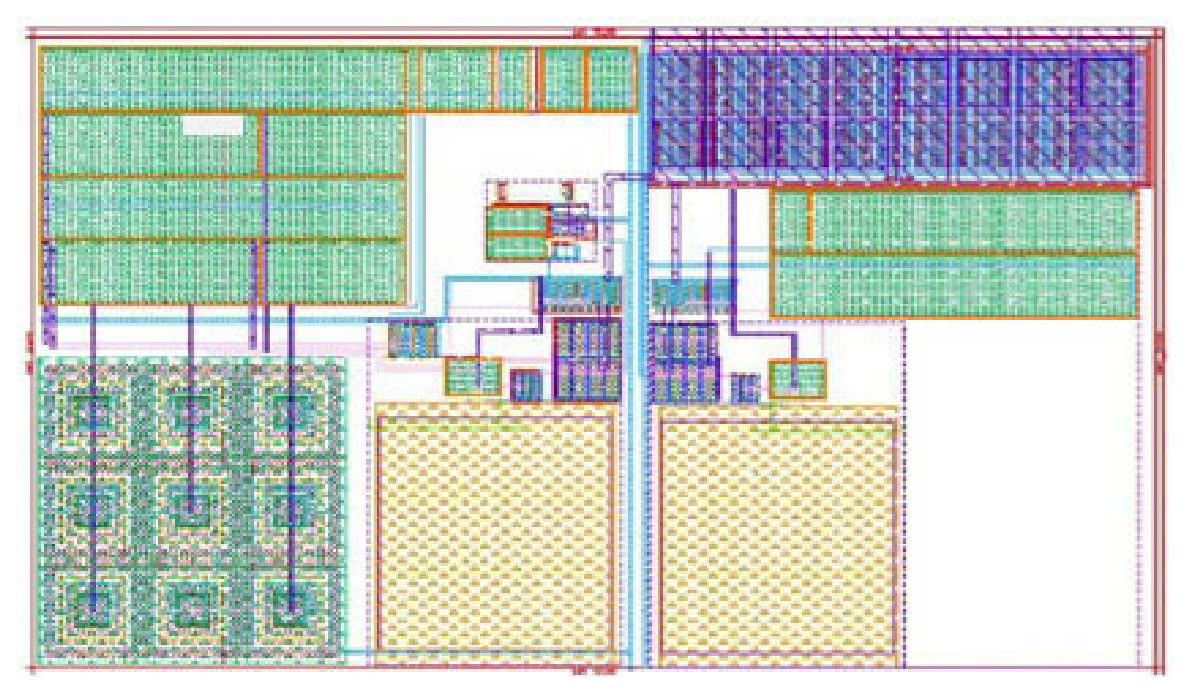
\includegraphics[width=\textwidth]{Fig/LDO_tsmc90_MR_1.eps}
        \caption{Original LDO layout on tsmc90nm}\label{fig:Original_LDO}
        \end{subfigure}
        \begin{subfigure}[t]{0.4\textwidth}
        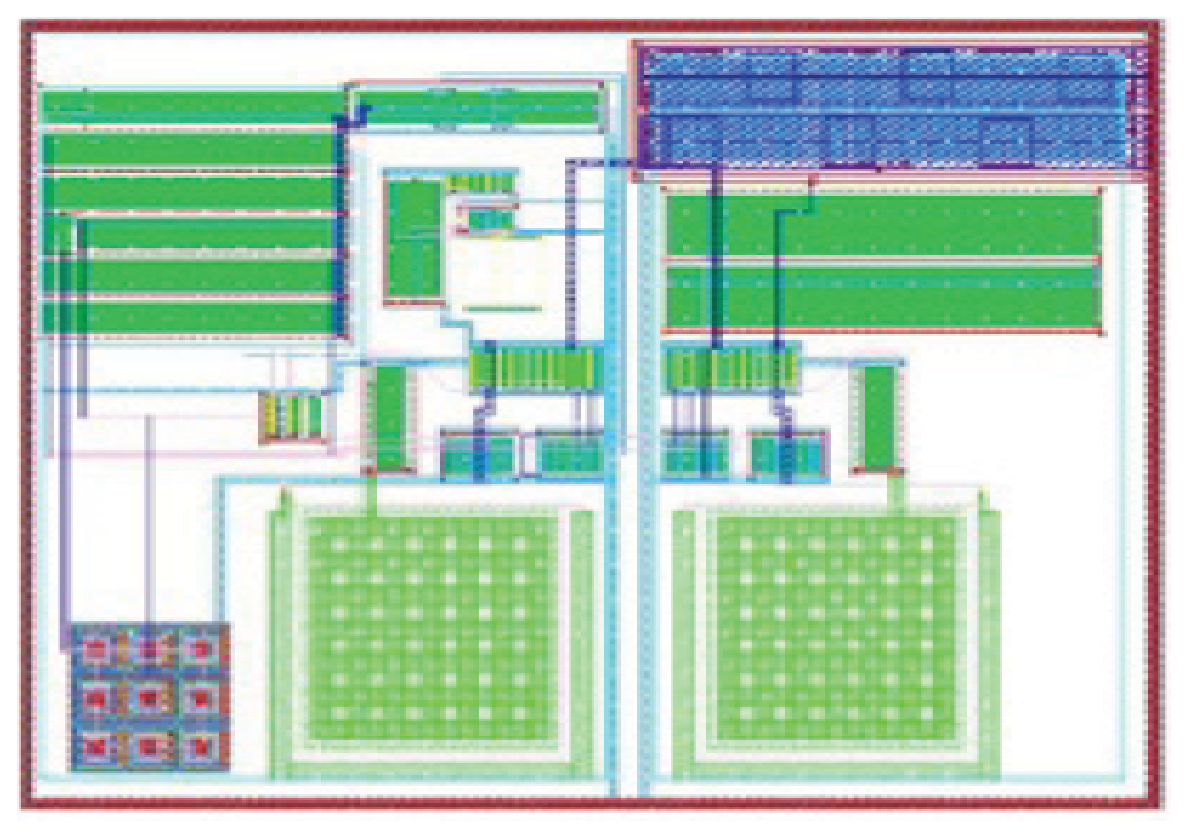
\includegraphics[width=\textwidth]{Fig/LDO_umc90_PlFuRtCDT_1.eps}
        \caption{\cite{msc-bhattacharya-tcad06}+\cite{Chin_DMR_ICCAD2013} on umc90nm}\label{subfig:LDO_umc90_PlFuRtCDT}
        \end{subfigure}
        \begin{subfigure}[t]{0.4\textwidth}
        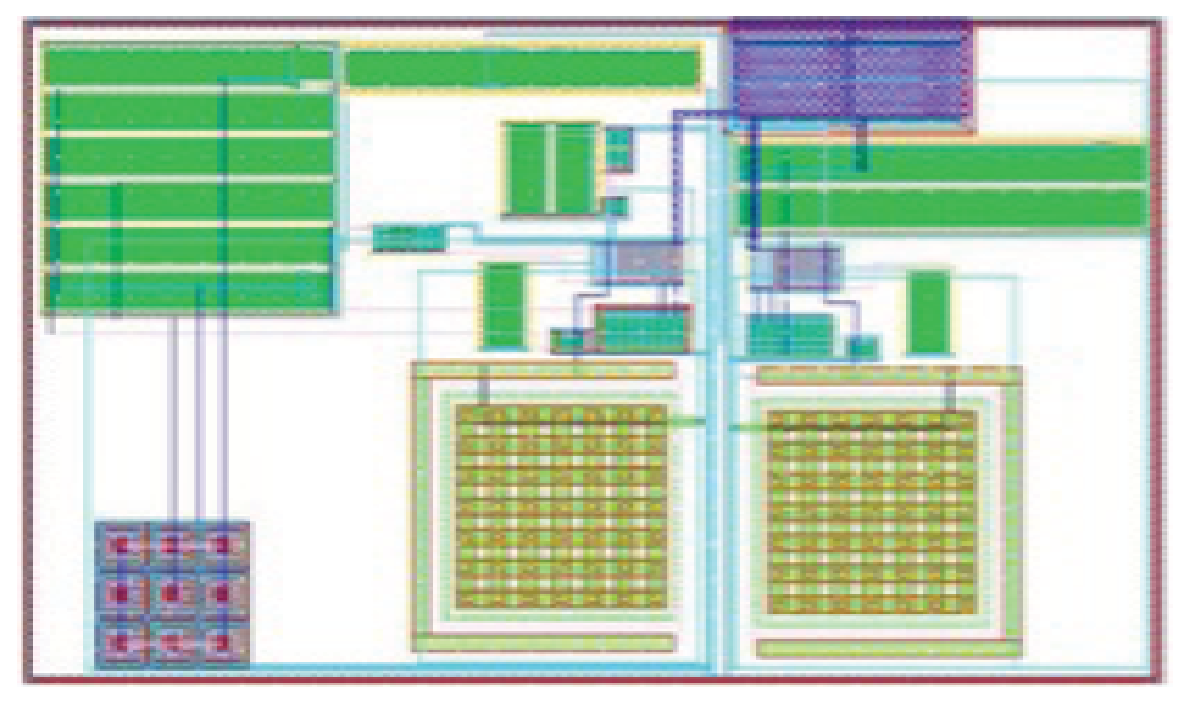
\includegraphics[width=\textwidth]{Fig/LDO_umc65_PlFuRtCDT_1.eps}
        \caption{\cite{msc-bhattacharya-tcad06}+\cite{Chin_DMR_ICCAD2013} on umc65nm }\label{subfig:LDO_umc65_PlFuRtCDT}
        \end{subfigure}
        \begin{subfigure}[t]{0.4\textwidth}
        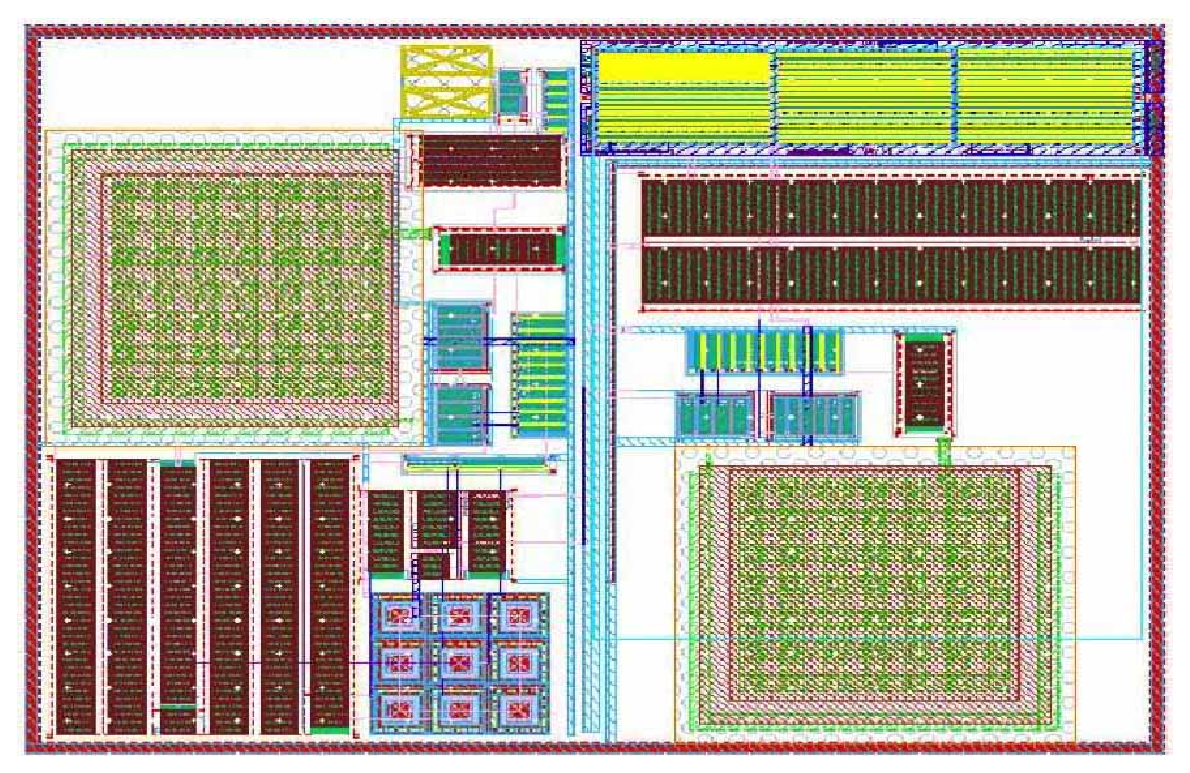
\includegraphics[width=\textwidth]{Fig/LDO_umc90_PlFxRtCDT.eps}
        \caption{Our approach on umc90nm }\label{subfig:LDO_umc90_PlFxRtCDT}
        \end{subfigure}
        \begin{subfigure}[t]{0.4\textwidth}
        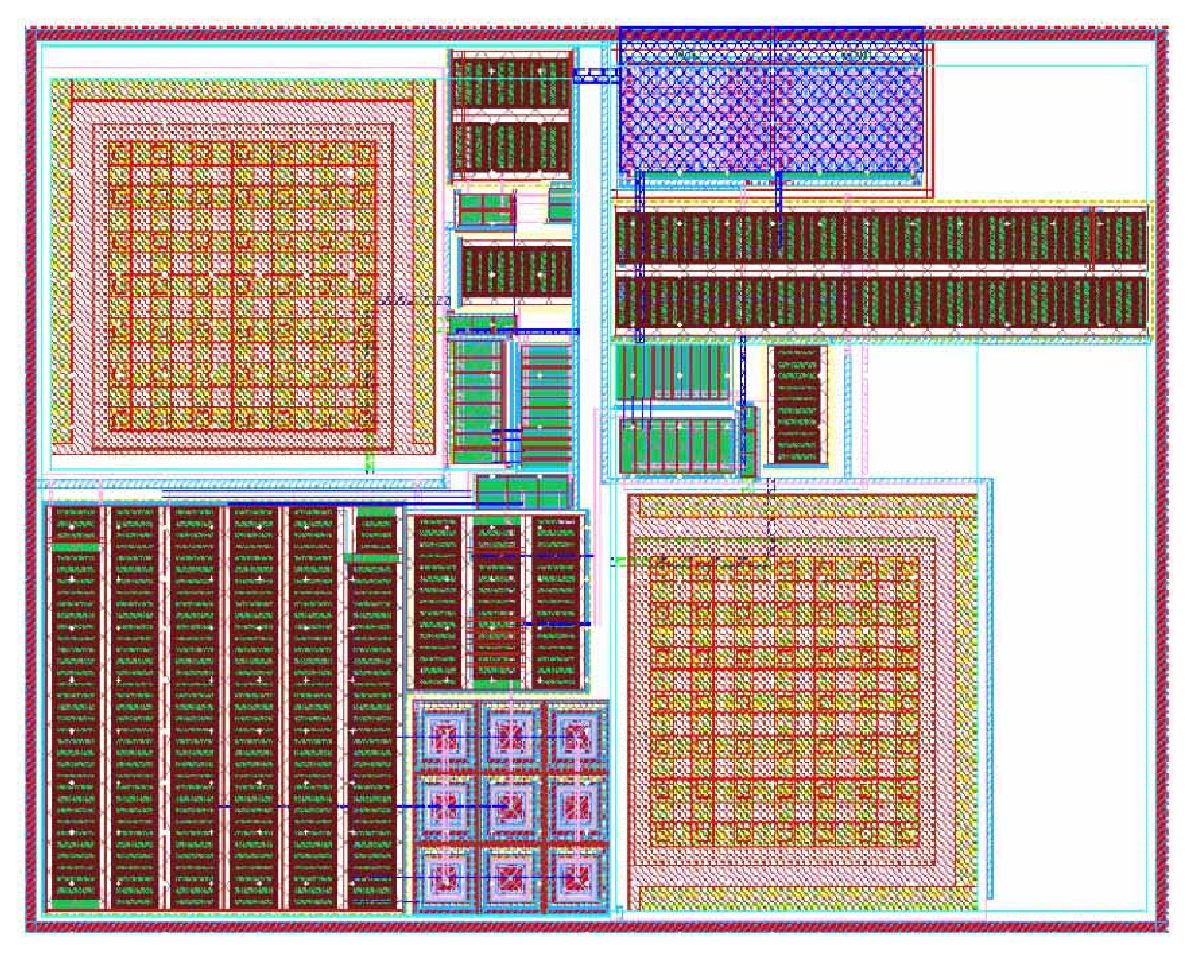
\includegraphics[width=\textwidth]{Fig/LDO_umc65_PlFxRtCDT.eps}
        \caption{Our approach on umc65nm }\label{subfig:LDO_umc65_PlFxRtCDT}  
        \end{subfigure}
      \caption{LDO from origin to migration with \cite{msc-bhattacharya-tcad06}+\cite{Chin_DMR_ICCAD2013} and our approach}\label{fig:LDO}
      \end{figure}


      

      In Table~\ref{table:HierProto}, row 3-14 show the feasibility on our approach for each technology with the simulation results, and all the testing circuit satisfy the performance specification. For umc90nm technology, our approach earns better performance on quiescent current, minimum $R_{on}$, $V_{out}$ settling time, temperature, power efficiency, $V_{drop-out}$, $\Delta V_{out-transient}$ and phase margin than \cite{msc-bhattacharya-tcad06}+\cite{Chin_DMR_ICCAD2013}. At the same time, for umc65nm technology, our approach earns better performance on dropout voltage, quiescent current, $Minimum R_{on}$, $V_{out}$ settling time, $\Delta V_{out-transient}$, open loop gain and phase margin. We can observe that even the other parts of simulation data are not notable. For the purpose to generate layout prototypes efficiently, a migrated layout with flexible placement topology dominate most of the performance metrics. Our approach framework accomplishes qualified layout results with higher productivity.

    
      For the reusability of the framework, we have collected further statistics in routing issues. As revealed in row 15-17 at Table~\ref{table:HierProto}, the overall WL, auto-gen WL and routing completeness represent the routing behavior among 5 layout results. In the original layout on tsmc90nm. The routing is accomplished manually with wirelength 2426.73$\mu m$, and the wirelength for the other two technologies with the same placement topology (\cite{msc-bhattacharya-tcad06}+\cite{Chin_DMR_ICCAD2013}) are 2122.814$\mu m$ and 1590.84$\mu m$. Meanwhile, our approach on umc90nm and umc65nm result in 1579.09$\mu m$ and 1308$\mu m$, respectively. We can observe that our approach takes more routing wirelength, but also earns more routing completeness with 78.8\% and 83.9\% on umc90nm and umc65nm. We can tell that the lost routing completeness rate is mostly made from the lost of triangles during {\it Crossing Graph Updating} in Section~\ref{sec:updateG}. The loss of triangles indicates the destruction of planar relationship. The more triangles miss, the more wires need to be reconnected. Even though our approach obtains worse routing completeness than \cite{msc-bhattacharya-tcad06}+\cite{Chin_DMR_ICCAD2013}, the performance is averagely better and the area is obviously compact than \cite{msc-bhattacharya-tcad06}+\cite{Chin_DMR_ICCAD2013}.

    In brief, the experimental results show that our approach with multiple placement topologies enlarges the solution space, CDT-based-migrated routing raises the routing reusability out of preservation and wire segment refinement explores the better performance. Meanwhile, the compelling speed-up of design time indicates the productivity for analog design.

  \section{Summary}\label{sec:RLPADMSum}

    This work introduces a rapid methodology for analog layout migration.The layout extraction and preservation is proposed to preserve placement and routing behavior with hierarchy and symmetry constraints. Based on the layout preservation, multiple layout solutions are efficiently generated by our migration with flexibility. A methodology for wire segment refinement is also delivered for better performance after migration.
    We validate the proposed method on a variable-gain amplifier, a folded cascode OpAmp and a low drop-out regulator.
    Experimental results demonstrate that our approach has the capability of preserving analog layout behavior of the reference layout. Moreover, the strategies with multiple placements generation and preserved routing provide better layout solution than previous approaches. The proposed migration flow generates layouts that have comparable performance with manual layout and state-of-the-art. In this way, our proposed work guarantees the routing reusability with at least 75\% completeness on wirelength and 80\% on wire segments of reconstructed routing and the productivity with at least 5 times speedup over manual layout.